\documentclass[a4paper,12pt]{article}
\usepackage[utf8]{inputenc}
\usepackage[pdftex]{color,graphicx}
\usepackage[english]{babel}
\usepackage[rflt]{floatflt}
\usepackage{tocloft}
\usepackage{tabularx}
\usepackage{thesis}
\usepackage[T1]{fontenc}
\usepackage{cite}
\usepackage{comment}

\myauthor{Karsten Köhler}
\mytopic{Semantic segmentation of terrain data using high-resolution orthophotos}

\begin{document}
    \mytitle

    \frontmatter
    \tableofcontents
    \section*{Abstract}
\noindent
The automated identification of emergency landing fields is a complex challenge which requires to process huge quantities of information. This thesis explores the use of convolutional neural networks to perform a classification of land use through semantic segmentation to support the identification process. For that, three popular reference architectures of U-Net~\cite{unet15}, FC-DenseNet~\cite{denseseg17} and W-Net~\cite{wnet17} are implemented and applied to this challenge. The experiments show that U-Net and FC-DenseNet achieve adequate segmentation results, while the unsupervised learning process of W-Net fails to learn a proper class differentiation. In a second step, several spectral vegetation indices are investigated whether they are applicable to further narrow down the number of suitable emergency landing fields. It is demonstrated that with the given dataset, the indices do not provide any meaningful information. Overall, this thesis offers a valuable contribution to the improvement of the automatic identification of emergency landing fields.
    \newpage

    \mainmatter

%    \lstinputlisting[caption={Some test code}, language=Python]{../python/code.py}

    \section{Introduction}
The failure of an aircraft's engine during a flight is a very serious event, even for experienced pilots. You have to make quick and informed decisions to handle the life-threatening situation properly. The motorized vehicle basically becomes a glider that's usually not able to keep flight height for a long time. With a very limited reach and a quite high sink rate, the most important task as a pilot is to find a runway close enough to your current location to perform an emergency landing.

There are various facts to be considered weather a specific runway is a viable option for an emergency landing. For example the distance to the runway is one of the more obvious parameters, but also things like wind conditions and gliding characteristics of the aircraft are important. However, the runway not only has to be within reach. Another condition is that you are able to approach the runway in a correct angle and with the correct altitude, either with a direct path or with some additional holding patterns. All in all, a good pilot has to take all these things into account while being in such a stressing situation.

It is no surprise that nowadays there are companies and researchers working on tools to support the decision-making process in many ways. One project called Emergency Landing Assistant (ELA) is developed at the FernUniversität Hagen in Germany~\cite{feu_fas}. The ELA uses various parameters like sink rates in both straight and curved flight paths, wind speed and direction and also different settings like flap positions. With that it calculates a recommended flight path to a nearby runway which is updated in real-time according to situational changes. Because of the precise simulation of real-world physics, this path tends to be much more accurate than a pilot's assessment, which is mostly based on experience and gut feeling.

Sometimes there is just no suitable runway that happens to be in reach for the emergency landing. As a last option to get down without crashing, the pilot has to find a spot in the landscape where he can safely touch down the airplane. Because this is such a high risk maneuver, it is only considered if there is really no other option. To reduce the risk of a crash it is essential to find an flat area with few obstacles. For that case, the ELA contains a module called Emergency Landing Field Identification (ELFI), which assists in finding zones suitable for an emergency landing in the wild~\cite{feu_elfi}. This thesis will work on improving said module using deep learning techniques with a publicly available dataset.

\subsection{Background}
An early version of ELFI used only LIDAR elevation data to detect emergency landing fields. As stated in~\cite{feu_elfi} they used high resolution height maps with an edge length of under 1m in the grid. A big drawback with elevation data is that you cannot rely on the data in every case. For example, water surfaces like lakes and large rivers are found to be perfect areas for an emergency landing. But in reality water has a much higher risk to land on compared to solid ground.

Furthermore, even height maps with very high resolution usually miss obstructions like power lines or small creeks. In the end this approach can give suggestions for considerable emergency landing areas, but the pilot still has to filter those results very closely. Additional data like remotely sensed images can be used in order to narrow down the number of potential emergency landing fields. With image data it is possible to recognize even very small objects as well as the surface conditions in the potential areas.

The latest version of the ELFI module already make use of this. However, the existing solutions are based on methods of traditional image processing only. With the recent success of machine learning and artificial neural networks, this topic offers encouraging opportunities to optimize the ELFI module. For that reason, also the FernUniversität Hagen conducts research on these approaches.

\subsection{Objectives}
The main objective of this thesis is to examine new ways of identifying and analyzing emergency landing fields with convolutional neural networks. The former methods are based exclusively on binary classification. With that, ELFI can only suggest potential areas and provide information such as inclination. To further support the pilot's decision making, this thesis investigates how to make more information available to the pilot by making use of high resolution orthographic photos. The District Government of Cologne provides a large dataset with digital orthographic imagery of Cologne and surroundings\footnote{For details see \url{https://www.geoportal.nrw/}.}.

To achieve the objective, we perform a semantic segmentation of the image data with convolutional neural networks. This process enables to distinguish between different zones like buildings, forest or water in an image. One of the main tasks is to investigate and evaluate certain reference architectures for the segmentation challenge. For this purpose, the reference architectures are first discussed in theory and then implemented and trained in practice. Based on their individual results, the suitability of the architectures is discussed concerning the identification of emergency landing fields.

In a second step, only those segmentation results are considered which are potentially suitable for an emergency landing (e.~g. excluding buildings). For these segments the density of the vegetation is to be analysed using spectral vegetation indices. Therefore, some indices are explored and their respective results on the given data set are demonstrated. Finally, it is discussed how such indices can be used for he classification of vegetation density in the context of emergency landing field identification.

\subsection{Outline}
\WIP{
\begin{itemize}
    \item Brief summary of all chapters and their content. This section will be written at the very end of the thesis.
\end{itemize}
}

\newpage
    \section{Literature Review}

\subsection{Types of Machine Learning Methods}
\begin{itemize}
    \item compare supervised vs unsupervised learning
    \item supervised learning will be used for land zone segmentation and vegetation analysis
    \item unsupervised learning might be used for dimensionality reduction
    \item this chapter only makes sense if unsupervised learning is put to good use
\end{itemize}

\subsection{Convolutional Neural Networks}

\subsubsection{Convolution}
\cite{DLbook16}
326: convolutional neural networks (CNN) are specialized kind of neural network for data with grid-like topology, for example images as 2D pixel grid. CNN are basically NN that use at least one convolutional layer.

330: NN use only matrix multiplication. meaning every output unit of one layer interacts with the all input units of the next layer. convolution leverages sparse interactions. for example images can have millions of pixels, but to detect edges it is enough to only look at a few pixels at a time. thus we can have a kernel smaller than the image size resulting in fewer parameters. This reduces memory requirements of the model and increases statistical efficiency.

331, 333: another advantage is parameter sharing. with matrix multiplication you usually have a weight matrix, where each value is used only once. convolution operation uses parameter sharing, because one kernel is applied multiple times on the same image. and since kernel is smaller than image, it again reduces number of parameters by a significant amount.

334f: due to parameter sharing, convolution operation is equivariant to translation. Meaning, if you move parts of the input convolution will still give you the same output, just with the moved detection. This is especially helpful for working with images, as object might be in different locations of the image, but should still be realized.

\subsubsection{Pooling}
\cite{DLbook16}
335: Pooling replaces output of certain location with a summary of the nearby outputs. Max Pooling reports the maximum value inside a rectangular neighborhood. Other functions: (weighted) average or $L^2$ norm.


\begin{figure}[h]
    \centering
    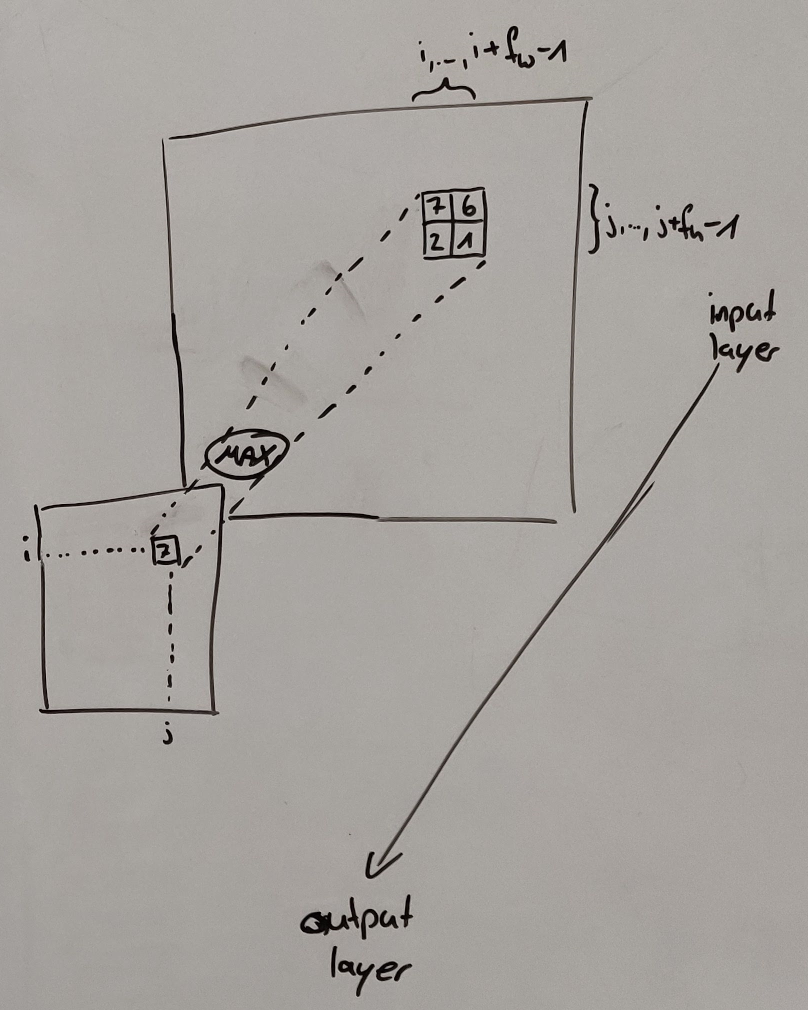
\includegraphics[width=0.8\textwidth]{images/maxpool}
    \caption{Max pooling \cite{stanford_convnet}}
    \label{fig:pooling}
\end{figure}

\cite{stanford_convnet}
Module 2: pooling layers between conv layers are common architecture. thereby you progressively reduce the spatial size and also number of params later in the net. pooling operates on all feature maps independently. For example pooling with kernel size 2x2 and stride 2 downsamples the input, so that 75\% of information is discarded.

Pooling layer are not trainable, because they compute a given function on the input elements. This function is oftentimes MAX function, also other variation like AVG oder L2-norm are used. However, pooling is configurable for the hyperparameters kernel size and stride.

\subsubsection{Others}
Batch Normalization, ReLU Activation, etc

\subsection{Reference Architectures}

\subsubsection{U-Net architecture}
\cite{unet15}
network architecture consists of a contracting path and an expansive path. contraction follows the typical architecture of convolutional network. repeated application of 3x3 convolutions, followed by ReLU and 2x2 max pooling. stride 2 for downsampling, features double for each contraction.
expansive path is upsampling followed by 2x2 convolution. also concatenation of the cropped feature map from the corresponding feature map from contraction path.
final layer is 1x1 convolution to map feature vector to desired number of classes. Demonstrated results with the EM segmentation challenge (\cite{isbi_challenge}), where they achieved very good results.

\begin{figure}[h]
    \centering
    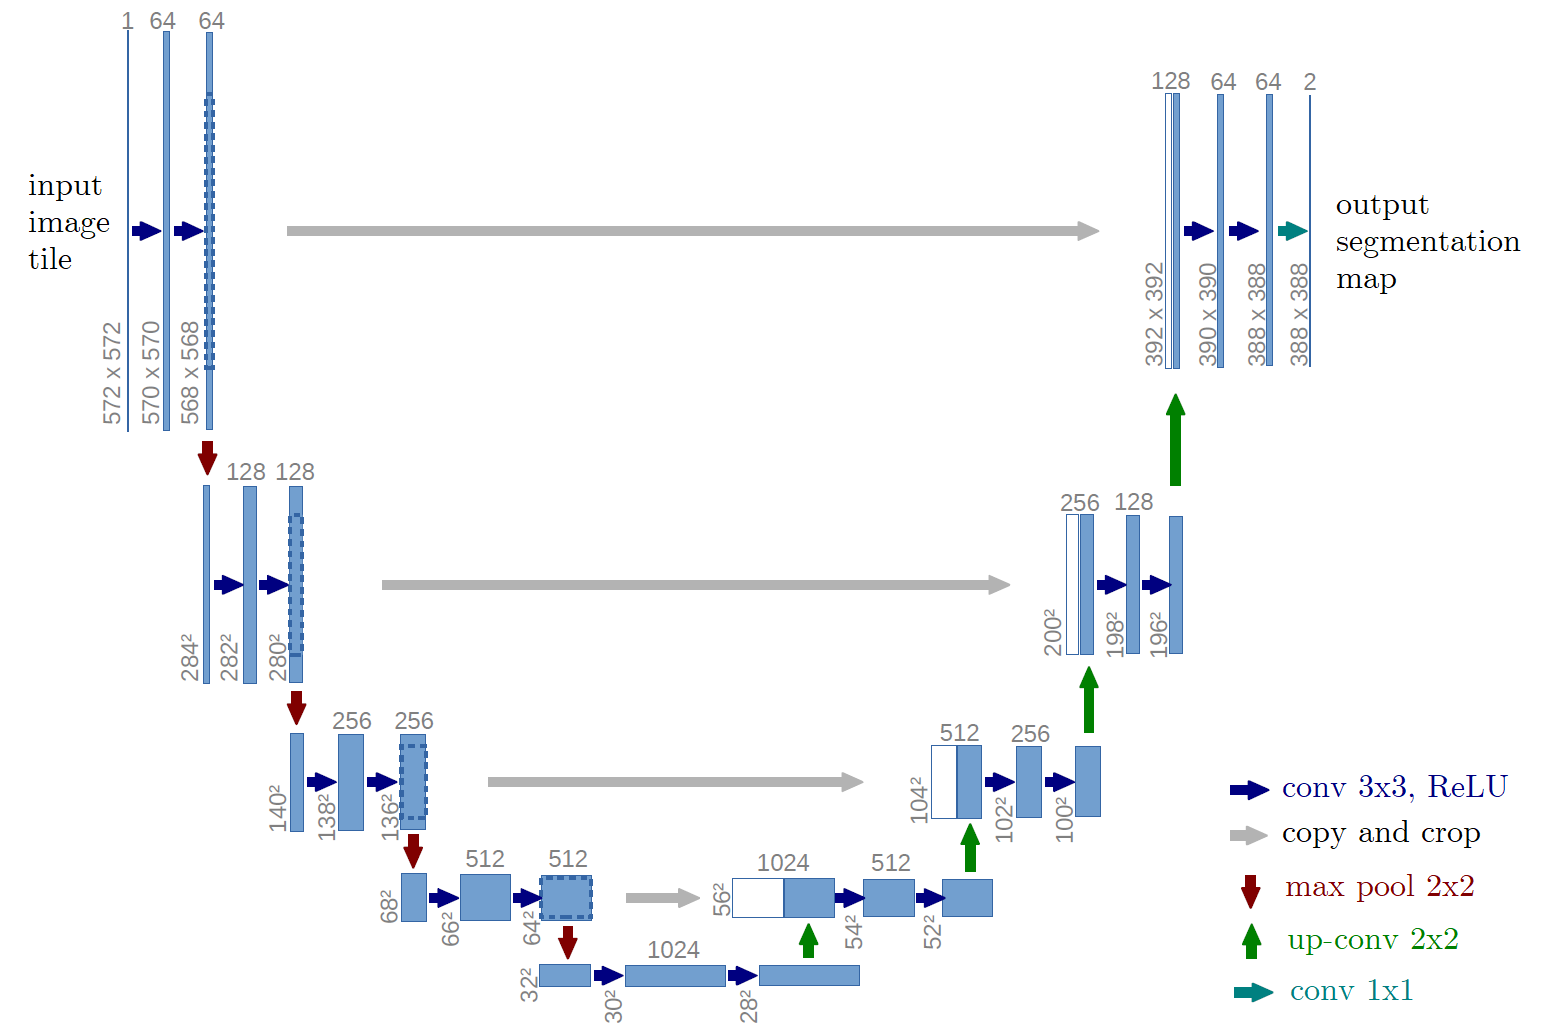
\includegraphics[width=0.9\textwidth]{images/u-net-architecture}
    \caption{U-Net Architecture \cite{unet15}}
    \label{fig:unet_architecture}
\end{figure}

\subsubsection{DenseNet Architecture}
\cite{densenet18}
NN architectures tended to get deeper and deeper. This brings problem of vanishing gradients because input data flows through so many layers. Different approaches to solve this. Authors of paper decided to connect all layers with matching feature map sizes. Features are combined by concatenation. This leads to many connections in a deep network, thus called Dense Convolutional Network (DenseNet).

Authors see layers as state of the network. For layer state to be accessible by next layers, the layer needs to pass the state. With their architecture, they differentiate between information coming from earlier layers and information being mined in the current layer. They keep layer narrow, each layer only adds small pieces of new information, existing information is not changed. All of that leads to having fewer parameters than traditional architectures.

Improved flow of gradients throughout the network. Every layer has access to original input signal and gradients from the loss function. Allows for even deeper architectures and prevents vanishing gradients. Make it easier to train the network.


\begin{figure}[h]
    \centering
    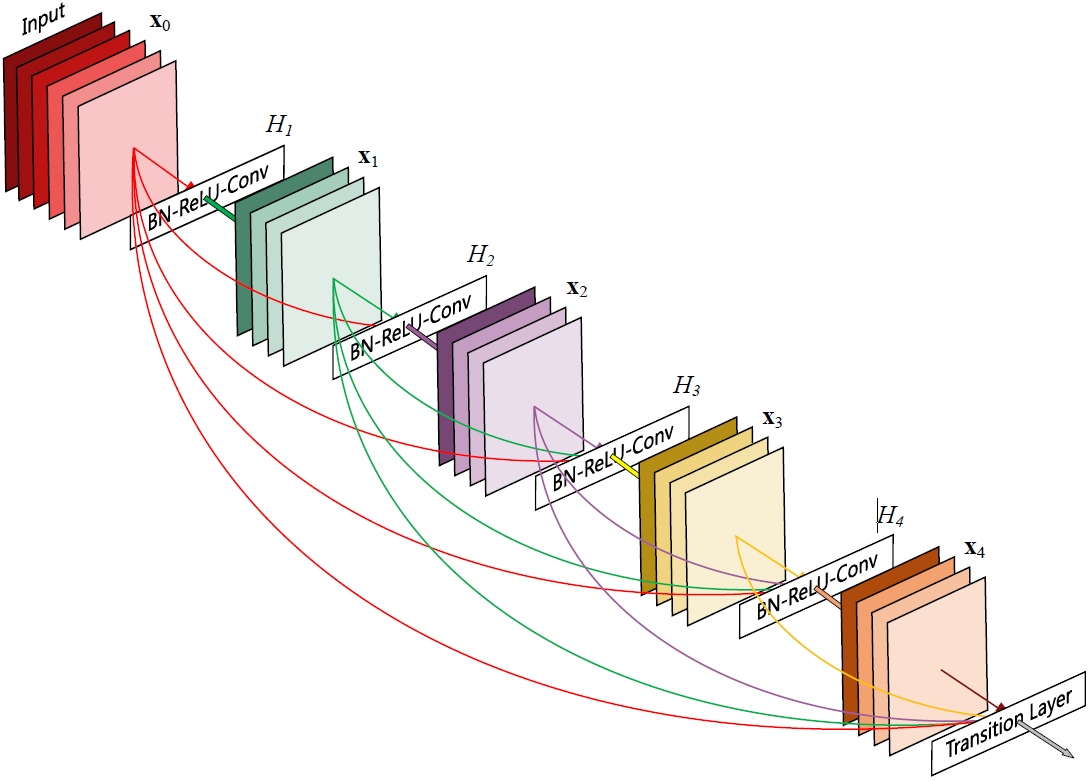
\includegraphics[width=0.9\textwidth]{images/dense-net-architecture}
    \caption{Densely Connected Convolutional Architecture \cite{densenet18}}
    \label{fig:densenet_architecture}
\end{figure}

\subsection{Architecture Comparison}
Interesting for architecture comparison: \cite{imseg_architecures}

\begin{itemize}
    \item point out the common characteristics and differences of the architectures
    \item compare use cases of the architectures and how they perform on them
\end{itemize}

\newpage
    \section{About the dataset}
% TODO: slower introduction into the section, talk about landing fields again
% TODO: elaborate why this specific dataset was used

The dataset which is used throughout this thesis is provided by the Ministry of the Interior of the State of North Rhine-Westphalia in Germany. With the platform GEOportal\footnote{available at \url{https://www.geoportal.nrw/}} they offer various types of maps, like topographical maps, elevation data and orthographical footage. Most of the data is available for free download in batches. The batches used in this thesis are released under the dl-de/zero-2-0 licence. This means that the data can be used for any purpose without any restrictions or conditions\footnote{see the full license text at \url{https://www.govdata.de/dl-de/zero-2-0}}.

For the purpose of this thesis there are two types of maps which prove useful. First, there is a map assembled of digital orthophotos (DOPs). A DOP is an aerial photograph of the surface of the earth. It is processed to hide effects like perspective distortions or topographic features of the landscape. Also it follows a specific map projection to denote the exact spatial extents of the photograph on the earth's surface. Because of that, DOPs are great to analyze terrain coverage and conditions. In section~\ref{sec:segmentation} DOPs are used to perform a semantic segmentation based on the terrain surface.

The second map explored in this thesis contains imagery obtained by near-infrared (NIR) spectroscopy. They are processed in the same way as the DOPs, so they are also projected onto the earth's surface with a specific map projection. NIR data is widely applied in agriculture to monitor the cultivation of herbal products like forages and vegetables. In this thesis the NIR imagery is used to approximate vegetation density for specific regions (see section~\ref{sec:vegetation_analysis}).

\subsection{Getting the dataset}
Both the DOP and NIR datasets are provided by the Ministry of the Interior in a few different ways. To get a quick overview, there is an online viewer for most of the map types available at \url{https://www.tim-online.nrw.de/tim-online2/}. For some specific maps like the DOPs they host a Web Map Tile Service, which allows to access the data with geographic information systems (GIS) like QGIS\footnote{QGIS is a free and open-source GIS application available at \url{https://qgis.org/}}. Since these options require a continuous network connection, it is preferred to get a local copy of the dataset and work with that.

For that purpose, the GEOportal has a separate download section. There you can choose the regions and map types you need and download them in a compressed bundle. The bundle contains map tiles in the JPEG 2000 file format. This is an image format that has a dense compression rate and directly contains the georeferencing for each tile. To have a wide range of terrain types with broad variety included, we use the data for the Municipality of Arnsberg and its surroundings. This concludes to a download size of $11.5~\text{Gigabytes}$ with around $248.49~\text{km}^2$ of terrain, where each pixel represents a $10\times 10~\text{cm}$ square in scale.
% TODO: JPEG 2000 not very widely accepted

It is possible to download both DOP and NIR data together in a single bundle. The JPEG files then contain four bands of pixel information. The first three bands make up the red, green and blue colors for the DOPs. And the last band provides the scalar output of the NIR spectroscopy scan.

% TODO: show some example images from the dataset, maybe later?
% TODO: demonstrate the limits of practical feasibility, maybe later?

\subsection{Preparing the dataset}
As a first step, the whole dataset is imported into a spatial database system. By doing that, it is very easy to export the data in various data formats and tile sizes required by the reference architectures (see section~\ref{sec:ref_archs}). PostgreSQL\footnote{see \url{https://www.postgresql.org/}} is a powerful open-source database system. Together with PostGIS\footnote{see \url{https://postgis.net/}}, a free and open-source extension for PostgreSQL, it is capable of performing spatial operations on image rasters and vector objects. For example, it adds database functions to merge raster tiles, calculate intersection regions or determine bounding boxes.
% TODO: created a database with postgis as single source of truth

The PostGIS installation contains a few shell tools to import data into the database. Unfortunately, they do not support the JPEG 2000 image file format. Before the import of the data can take place, it has to be translated to one of the supported formats first. One of the most widely used formats is GeoTiff. The Tiff file standard is great, because it consists of a baseline section which contains the image information, and a meta section which can contain all kinds of meta information. For example, it can be used to store georeferencing information, which PostGIS is able to use for importing GeoTiff files.

To convert the files from JPEG 2000 to GeoTiff, we use the \emph{Geospatial Data Abstraction Library} (GDAL). This is a tool collection which acts as an abstraction layer for various geospatial data formats. It also includes a shell tool to translate several georeferenced image file formats, including JPEG 2000 and GeoTiff. Listing~\ref{lst:jp2_to_tif} in appendix~\ref{app:code} shows a bash script using the \texttt{gdal\_translate} tool to convert all the JPEG 2000 files to the GeoTiff format.

With the files in GeoTiff format it is now possible to use the \texttt{raster2pgsql} tool to import them into a PostGIS raster table. The whole import process is automated with a Python script (see listing~\ref{lst:tif_to_raster} in appendix~\ref{app:code}). It assumes that there is a database called \texttt{dop10rgbi\_nrw} with the PostGIS extension enabled.

In the first step, the script creates two database tables named \texttt{dop\_rgb} and \texttt{dop\_nir}. The \texttt{dop\_rgb} table has a PostGIS raster column with three raster bands to hold the color information for the DOPs. Simultaneously, the \texttt{dop\_nir} table also has a PostGIS raster column with only one raster band for the NIR values. It is reasonable to separate the color and NIR values as they will be used for different tasks later on.

After the tables are created, the script loops through all the GeoTiff files and calls the \texttt{raster2pgsql} tool for every single one. That call returns some SQL insert statements enriched with the raster information in a binary representation. To execute those statements, it is possible to simply pipe the output of \texttt{raster2pgsql} into a \texttt{psql} command which is connected to the database.

The \texttt{raster2pgsql} tool provides a lot of arguments to properly configure the import of the data. Obviously it needs to know the name of the file to import and the name of the database table to insert the data to. For performance reasons it is very important to set an appropriate tile size for the raster. The original tile size of the GeoTiff files ($10000\times 10000$ pixels) was assessed to be too large. After some experiments, a tile size of $1000\times 1000$ pixels was found to work best for both the initial import and the later processing of the raster.

Another major configuration is the spatial reference id (SRID). It also has to be passed as an argument, to ensure the data is imported correctly. The SRID indicates the map projection that is used to map the raster to the earth's surface. The dataset is provided with the SRID 25832. This SRID does not cover the entire globe, but only a rectangular area on the European continent. Therefore it offers a high precision (without too much distortion) in that area and is widely used for maps in Central Europe.

After all GeoTiff files are imported, the Python script creates a Generalized Search Tree (GiST) index for both tables. This takes into account the spatial character of the data and thus speeds up spatial queries (like merging, intersecting) on the tables significantly. For the same reason, the Python script also enforces some constraints on the raster columns of the tables. This makes sure that all the raster tiles share common properties like tile size, SRID or the number of raster bands.

As a last step of the Python script, it creates one last table named \texttt{geom\_bounds}. This table holds a single PostGIS geometry object defining the exact boundaries of the raster tiles. That allows for a quick way to calculate if a given region is included in the spatial extents of the raster without having to process the whole raster table all the time.

Figure~\ref{fig:dop_rgb_all} shows the color bands of the whole dataset and its location in Germany. To show the granularity of the data, one region is enlarged and shown in full resolution. One pixel in the dataset represents $10\times 10$ decimeters in real-world scale. As can be seen in figure~\ref{fig:dop_rgb_all}, it is easily possible to detect objects like trees, cars or buildings with such a high resolution. Therefore, the data provides sufficient information for the segmentation of land usage.

% TODO: adjust figure, show map of Germany, zoom to whole dataset, then zoom to high-resolution tile
\begin{figure}[h]
    \centering
    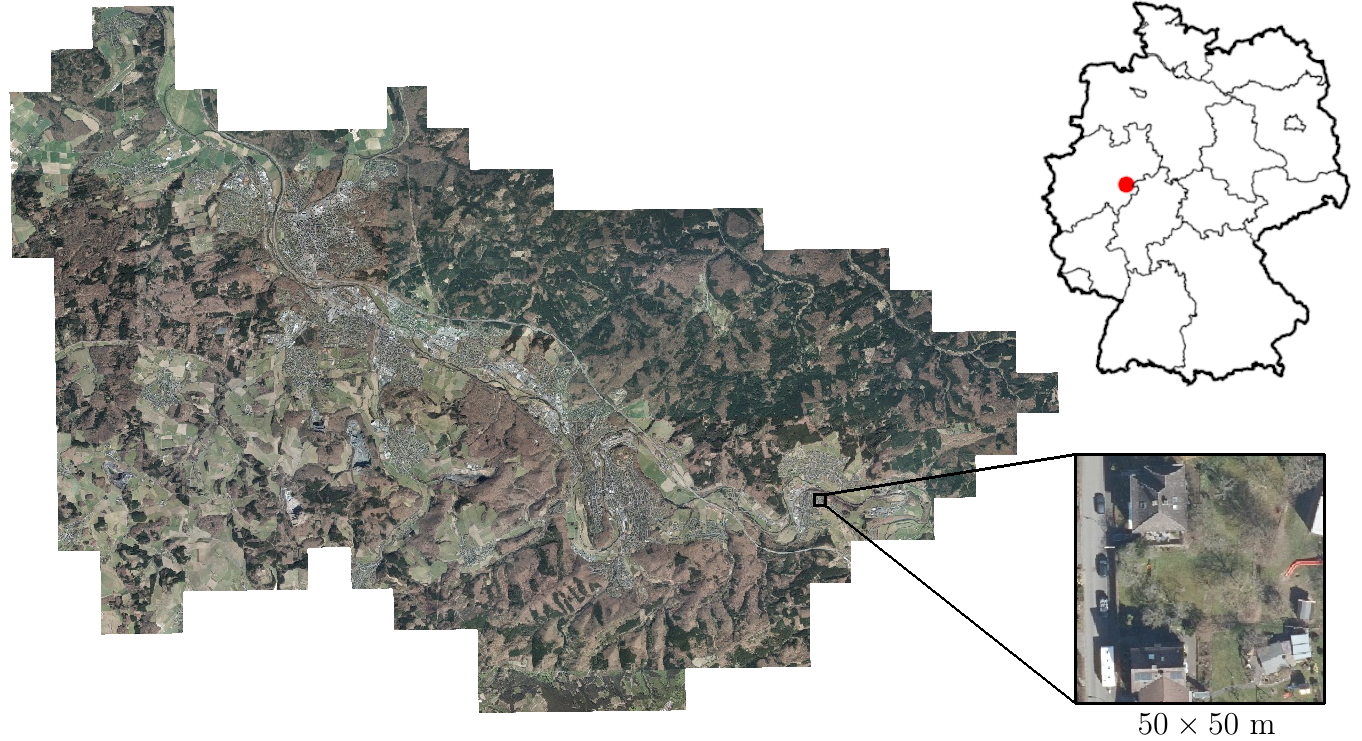
\includegraphics[width=\textwidth]{images/dop_rgb_all}
    \caption{The DOPs in the dataset}
    \label{fig:dop_rgb_all}
\end{figure}

\subsection{Preparing the labels}
As explained in section~\ref{sec:dl_paradigms}, for supervised training you need to provide the model with a pair of input and expected output. The DOPs explained in the previous section function as input for the model. To train the model for segmentation, another prerequisite is to have some segmentation examples prepared. Usually this task is done manually by lining out the segments of a tile and then assigning a category to each segment.

To reduce the amount of work, we use another dataset from the GEOportal called Digital Basic Landscape Model~\cite{base-dlm20}. It describes topological features of the landscape in a vector data format. Besides other things like \WIP{points of interest}, it includes regions categorized by their respective land use. The dataset is available for free download and also permits any use within the dl-de/zero-2-0 license. With some transformation the data fits perfectly for the use as labels during the training of a model.

The categorized regions are provided as Shapefiles. Shapefile is a specific data format for vector-based geospatial objects. To have all data in a single source system, the Shapefiles are imported into the PostGIS database. This also makes it easier to export the segmentation information later on for different tile sizes. Again, the import process is automated with a Python script (see listing~\ref{lst:tif_to_raster} in appendix~\ref{app:code}).

PostGIS includes a tool called \texttt{shp2pgsql} to import Shapefiles into a database table with a PostGIS geometry column. It takes into account all the metadata that is listed in the Shapefile and creates separate columns for those values. The Python script loops over all the required Shapesfiles and calls the \texttt{shp2pgsql} tool passing some arguments like the target SRID. At first, each file is imported in its own database table. This is because each file contains a specific set of meta information resulting in different table layout for each file. The categorized regions are now represented as PostGIS geometry objects.

The original Shapesfiles enclose all regions of the State of North Rhine-Westphalia. Since the DOP und NIR datasets only consist of a smaller subregion, all geometry objects are cropped to that subregion in the next step. Geometry objects that are located outside of the boundaries are dropped entirely. During this process, the tables of the different Shapefiles are merged into one single table. This resulting table has columns for an internal id, the object type, a textual object description and for the geometry object itself. As all the other meta information contained in the Shapefiles is not needed, it is dropped in this step.

The Shapefiles contain a few more categories than the segmentation in this thesis aims for. For example, the difference between industrial zones and housing zones is negligible for the purpose of emergency landings. Thus, the categories are mapped to six predefined supercategories:
\begin{itemize}
  \setlength\itemsep{1mm}
  \item water
  \item buildings
  \item agriculture
  \item forest
  \item urban greens
  \item traffic
\end{itemize}
The mapping between the categories of the Shapefiles and the chosen supercategories is to be found in table~\ref{tab:category_mapping}.

\begin{table}[]
\centering
\small
\caption{Mapping from Shapefile objects to segmentation categories}
\label{tab:category_mapping}
\begin{tabular}{|l|l|l|l|}
\hline
\textbf{Shapefile} & \textbf{Object Code} & \textbf{Object Description}    & \textbf{Segmentation Category} \\ \hline
gew01\_f           & 44001                & running water                  & water                          \\ \hline
gew01\_f           & 44005                & harbor dock                    & water                          \\ \hline
gew01\_f           & 44006                & stagnant water                 & water                          \\ \hline
sie02\_f           & 41007                & specialized regions            & buildings                      \\ \hline
sie02\_f           & 41009                & cemetery                       & urban greens                   \\ \hline
sie02\_f           & 41002                & industrial zone                & buildings                      \\ \hline
sie02\_f           & 41010                & housing zone                   & buildings                      \\ \hline
sie02\_f           & 41008                & sports, recreation          & urban greens                   \\ \hline
sie02\_f           & 41005                & quarry, surface mining         & buildings                      \\ \hline
veg01\_f           & 43001                & agriculture                    & agriculture                    \\ \hline
veg02\_f           & 43002                & forest                         & forest                         \\ \hline
veg03\_f           & 43003                & woody, undergrowth             & forest                         \\ \hline
veg03\_f           & 43004                & heath                          & forest                         \\ \hline
veg03\_f           & 43007                & uncultivated zones             & agriculture                    \\ \hline
ver01\_f           & 42009                & urban squares                  & traffic                        \\ \hline
ver01\_f           & 42001                & road traffic                   & traffic                        \\ \hline
ver03\_f           & 42010                & rail traffic                   & traffic                        \\ \hline
\end{tabular}
\end{table}

The last step is to merge all geometry objects of the same category. I. e. the final table only contains six geometry objects, one for each category. This was done for convenience and performance reasons, since almost all operations performed on this table include some way of merging the geometry objects of the same category.

Figure~\ref{fig:dop_label_all} depicts the segmentation for the whole dataset with a color encoding. The most dominant categories are clearly forest and buildings. Water and traffic zones only take up a very small area and both are barely visible because of the scale of the illustration. The imbalance of the categories is an issue which is further addressed in section~\ref{sec:dataset_considerations}

% TODO: show mapping from categories to colors
\begin{figure}[h]
    \centering
    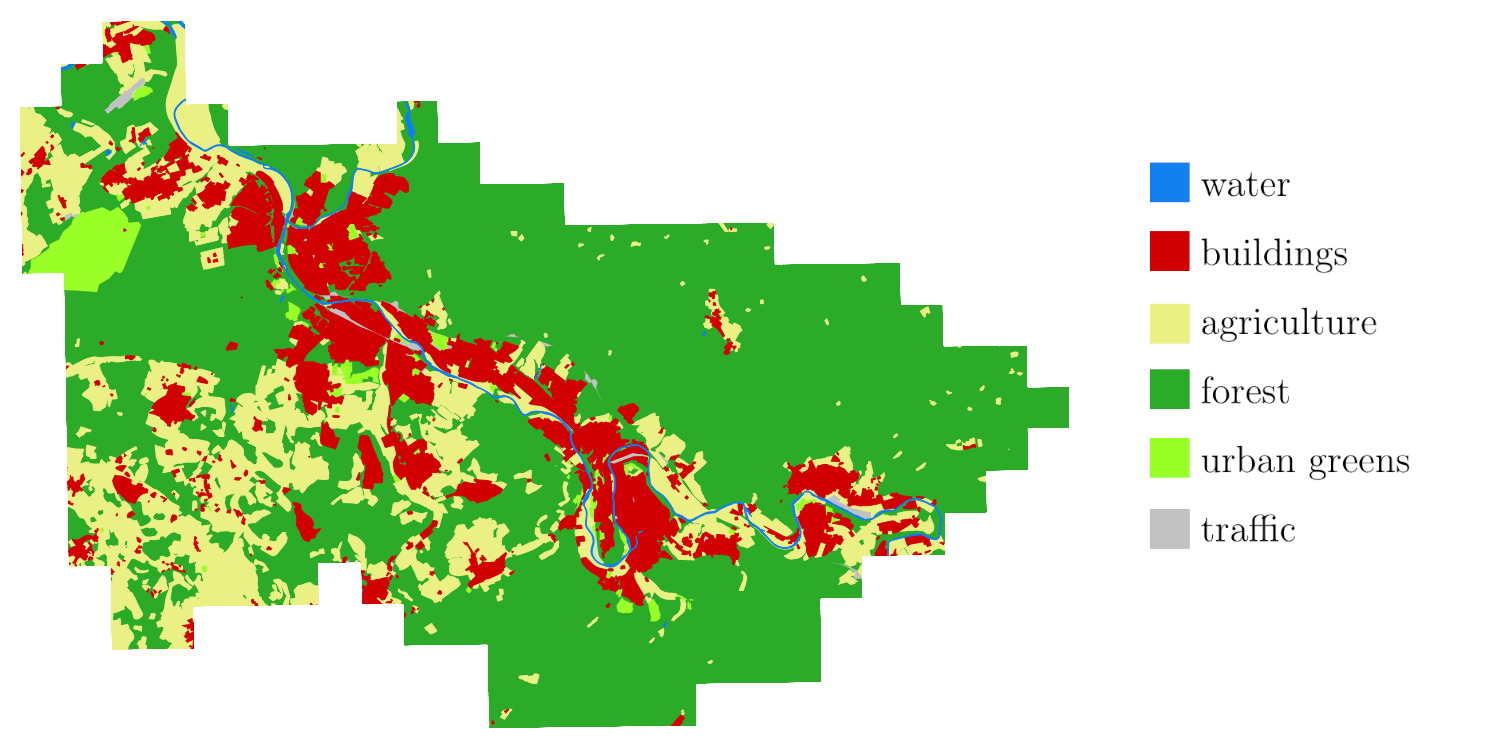
\includegraphics[width=\textwidth]{images/dop_label_all}
    \caption{The labels in the dataset}
    \label{fig:dop_label_all}
\end{figure}

\subsection{Export images for training}
% TODO: confirm numbers for training/querying time
At this stage, all the data required for the training of network models is contained in the PostgreSQL database and can be queried in regions of arbitrary tile size. While it is possible to query each tile live during training, this is highly inefficient. Since the same data is fed into the network multiple times, the same query result would have to be computed multiple times during a training run (i.~e. once per epoch). Also, doing a full round of backpropagation with a single tile is by far faster than executing a query for a single tile. Depending on the architecture of the network and the available hardware, a single pass of backpropagation usually takes around \WIP{$500~\text{ms}$} at most. Compared to that, the database query for a single tile measures on average to \WIP{$x~\text{ms}$}.

One common way to use more of the available processing power for the actual training, all tiles are precomputed and saved in well-sized batches on a hard drive. That way, they only need to be loaded into memory and can then be used directly. However, depending on batch size and the hard drive's reading speed this might leave the hard drive as bottleneck. In the end, the process of feeding the data into the network is a balancing act between factors such as data compression, preprocessing pipelines and hardware availability.

% TODO: reference the correct section
For this thesis, the data is exported from the database and saved as image files in PNG format. This format offers a good tradeoff between file size on the hard drive and processing time required to decode the data. The width and height of the images depends on the shape of the input layer of the network to train and will thus be discussed later on in \WIP{section~\ref{sec:segmentation}}. It is possible to store each tile in a separate file, but in general, the tiles are so small that this would not be very efficient. That way, hundreds of file handles will be opened and closed each second during training, which might cause performance issues with the operating system. Instead, multiple tiles are arranged in a grid layout in a single image file. This only requires an array split operation after reading a file, which is computationally cheaper than dealing with lots of file handles.

The PNG image format is used for both the DOP footage and the segmentation labels. For the DOPs this works great, because they contain three color bands that can be stored in the RGB channels of a PNG file. It was found to be better for training if the input values are normalized to range $[0, 1]$ before feeding them to a network \WIP{SOURCE}. Since the PNG files use 8 bit per color, this normalization can be achieved by dividing the color values by $255$.

In the image files the labels use color-encoding to differentiate between the categories. However, this is a bad representation for training, since the distance of the colors in the color space does not correlate with the similarity of the terrain types. This means the colors chosen for the categories would influence the segmentation predictions made by the network. Thus, after reading a label from a PNG file it is transformed to one-hot encoding. In one-hot encoding, each pixel is assigned a vector with one value per category. The value for the category is set to $1$ if the pixel belongs to that specific category, and $0$ otherwise. That way, the distance between the categories is equal for each pair of categories, i.~e. there is no correlation between categories. The translation from color-encoding to one-hot encoding is done by simply mapping the color vectors to their respective one-hot encoded representation.

While the exact tile and label size depends on the network architecture, there is a general process how the image tiles are extracted from the database. This process is automated with multiple Python scripts (see \WIP{appendix~\ref{app:code}}) . The first step is to define the bounding boxes of all tiles for a specific network architecture in a separate table within the database. Each bounding box is represented by a rectangular PostGIS geometry object. It is important to line up the tiles precisely with the DOP raster, so that the raster pixels are not distorted or cut off during the export. This does not matter for the labels, because they are stored in a vector format which is not based on pixels.

To extract the image files for those tile definitions, one straightforward way would be to join the raster table \texttt{dop\_rgb} with tile table containing the tile geometries using the PostGIS \texttt{ST\_Union} and \texttt{ST\_Intersection} functions. However, this was found to take a very long time to compute. Instead, a geospatial visualization software called \emph{QGIS} was used to do those computations. It offers a Python API which allows to run batch exports of a PostGIS raster table according to the bounding boxes defining the tiles.

\WIP{
with all the tiles outlined, it is possible to generate images/label now. This can be done using the PostGIS raster bands and merging/intersecting them in a smart way. Still this would take a long time. It was found that this process is faster when using QGIS, an application to show/render geospatial data. it has a python API, allowing to run automatized exports. This is the way we go, rendering all tiles with image data and also all tiles with the segmentation info.

unfortunately, for rendering the segmentation info QGIS does interpolation for borders between segments. This is not what we want, because for the labels each pixel should clearly belong to one category. Thus, we have another script to correct the rendered labels. this just takes the interpolated pixels and assigns them to one of the adjacent categories in the label. After that, the images and labels are ready to use.
}

\begin{figure}
    \newcommand{\DopLabelImageWidth}{0.23\textwidth}
    \centering
    \hfill
    \begin{subfigure}{\DopLabelImageWidth}
        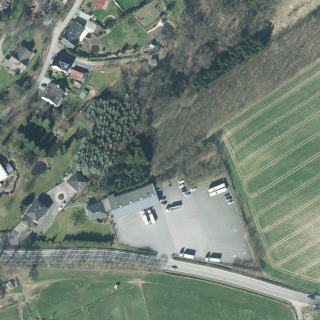
\includegraphics[width=\textwidth]{images/186_image}
    \end{subfigure}
    \hfill
    \begin{subfigure}{\DopLabelImageWidth}
        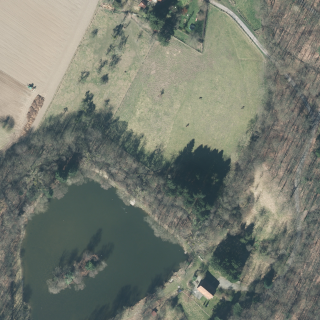
\includegraphics[width=\textwidth]{images/583_image}
    \end{subfigure}
    \hfill
    \begin{subfigure}{\DopLabelImageWidth}
        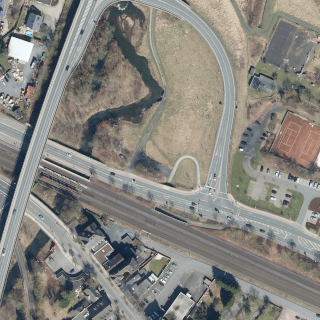
\includegraphics[width=\textwidth]{images/2281_image}
    \end{subfigure}
    \hfill
    \begin{subfigure}{\DopLabelImageWidth}
        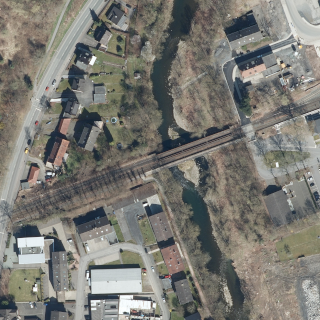
\includegraphics[width=\textwidth]{images/3589_image}
    \end{subfigure}
    \hfill

    \vspace{3mm}

    \hfill
    \begin{subfigure}{\DopLabelImageWidth}
        
\includegraphics[width=\textwidth]{images/186_label}
    \end{subfigure}
    \hfill
    \begin{subfigure}{\DopLabelImageWidth}
        
\includegraphics[width=\textwidth]{images/583_label}
    \end{subfigure}
    \hfill
    \begin{subfigure}{\DopLabelImageWidth}
        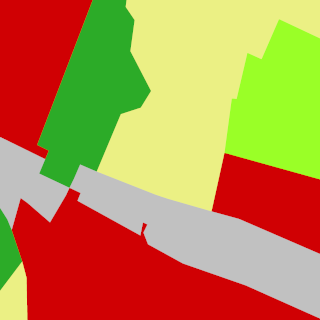
\includegraphics[width=\textwidth]{images/2281_label}
    \end{subfigure}
    \hfill
    \begin{subfigure}{\DopLabelImageWidth}
        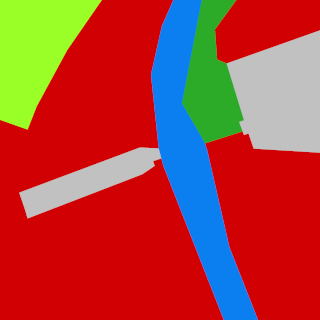
\includegraphics[width=\textwidth]{images/3589_label}
    \end{subfigure}
    \hfill

    \caption{Some image tiles with the respective labels}
    \label{fig:dop_with_labels}
\end{figure}

\subsection{Considerations about the dataset}
\label{sec:dataset_considerations}
\WIP{
shapes in the labels are not super accurate. on macroscopic point of view, they cover all segments on large areas. but borders between segments are oftentimes poorly represented. meaning transition between forest and agriculture or coastal line along rivers modelled very roughly. to get really good training results one should preferably use pixel-perfect labels. for purpose of this thesis, where the goal is to identify suitable emergency landing areas, this might not be a big issue as we are looking for open wide areas and don't care to much about perfect borders. But anyway, keep it in mind during model training.
% TODO: show images/labels to support this argument

Another thing is distribution of segmentation classes in the dataset. table~\ref{tab:seg-breakdown} shows relative coverage of the area with the categories. you can see that around 65\% of the data set consist of forest. On the other hand the area of traffic and water combined is still under 1\%. In general, this is really bad for training DNNs. Will lead the network to predicting forest way more often than water/traffic. For optimal results the categories should be well balanced inside the training dataset. So this is also a point to consider later on.
% TODO: find a paper to support this argument
}

\subsection{Choose the test dataset}
\WIP{

}

\begin{table}[h]
\centering
\begin{tabular}{|l|r|r|r|r|r|}
\hline
\multicolumn{1}{|c|}{\textbf{segment}} &
  \multicolumn{1}{c|}{\textbf{total $m^2$}} &
  \multicolumn{1}{c|}{\textbf{total rel. $m^2$}} &
  \multicolumn{1}{c|}{\textbf{test $m^2$}} &
  \multicolumn{1}{c|}{\textbf{test rel. $m^2$}} &
  \multicolumn{1}{c|}{\textbf{test / total}} \\ \hline
forest       & 162,554,698 & 65.40\% & 17,430,019 & 61.63\% & 10.72\% \\ \hline
buildings    & 30,821,514  & 12.40\% & 3,827,202  & 13.53\% & 12.42\% \\ \hline
urban greens & 5,715,026   & 2.30\%  & 716,624    & 2.53\%  & 12.54\% \\ \hline
agriculture  & 47,331,698  & 19.04\% & 5,898,601  & 20.86\% & 12.46\% \\ \hline
water        & 1,344,467   & 0.54\%  & 273,114    & 0.97\%  & 20.31\% \\ \hline
traffic      & 788,878     & 0.32\%  & 135,977    & 0.48\%  & 17.24\% \\ \hline
\end{tabular}
\caption{Breakdown of segments}
\label{tab:seg-breakdown}
\end{table}

\newpage

    \section{Segmentation of land zones}
\label{sec:segmentation}

Now that all fundamentals are covered, this chapter focuses on the implementation of the neural networks. Each reference architecture from section~\ref{sec:ref_archs} will be trained and evaluated with the original hyperparameters first. Afterwards, slight modifications are applied to the architectures, to look for optimization opportunities for the task at hand.

All implementation are done in Python with the popular Keras framework backed by TensorFlow~\cite{tf_whitepaper15}. It is a well established framework with extensive tooling, lots of documentation and a great open-source community. Also it is proven to be production-ready by a broad variety of companies for all kinds of tasks\footnote{Case studies can be found at \url{https://www.tensorflow.org/about/case-studies}}. More information about tools and hardware used throughout this thesis is listed in appendix~\ref{app:tools_hardware}

\subsection{Preparing the training and test dataset}
\label{sec:prepare_train_test}

Since the goal is to have a model that is able to generalize, it is recommended to measure its performance on data that it has not seen during training. Therefore, the dataset is split in two disjoint sets of data called \emph{training set} and \emph{test set}~\cite[p.~101f]{DLbook16}. During training, only samples from the training set are presented to the model. Afterwards, the performance is measured with samples from the test set. That way, models which just memorize the training examples perform rather bad compared to models which learn features on a generalized level.

The test set should only be used to evaluate the performance, but not decide on hyperparameters or architecture of the model. Otherwise, the model may become too closely aligned with the test set, i.~e. it is no longer possible to evaluate the generalization ability of the model with it. For such decisions another split of the training set is made, which is then called \emph{validation set}~\cite[p.~119]{DLbook16}. This set is used to estimate the generalization error during training and optimization without consulting the test set. Only after all optimizations have been done and no further changes to the model are planned, the test set is used to evaluate the final performance of the model.

There are many ways to pick the samples for the test and validation sets. \cite{val_split18} provides an insight into commonly used techniques. For this thesis, the test set respects the class imbalance that is found within the full dataset (see section~\ref{sec:dataset_considerations}). This is to achieve fair evaluation results which are not biased by any particular class. For each class, $10\%$ of the samples containing this class were chosen and added to the test set. The remaining samples are randomly distributed among training and validation set at a ratio of $9:1$.

\subsection{Tackling class imbalance}
\label{sec:class_imbalance}

As already expressed in section~\ref{sec:dataset_considerations}, there is a large imbalance between the segmentation classes in the dataset. This can lead to undesirable biases when training a model with such a dataset. For example, if the model predicts the \texttt{forest} class for every pixel all the time, the categorical accuracy would be at $65\%$ measured over the entire dataset. While this number does not sound too bad, the actual segmentation results would be useless.

There are some techniques to tackle the issues that come with an imbalanced dataset. One approach is to add class specific weights for the loss function during training~\cite{class_imbalance19}. The weights will affect the outcome of the loss function and therefore also the gradients during backpropagation. They are assigned antiproportionally to the distribution of the classes, i.~e. overrepresented classes are given small weights and underrepresented classes are given big weights. This has the same effect as duplicating the underrepresented samples in the training set, but it is computationally more efficient.

One major challenge is to find appropriate class weights, so that the imbalances are minimized as much as possible. For the given dataset, this can be done by taking into account the respective surface area for each class. Many different sets of class weights were tested, but none of them proved to be well suited. All trained models ended up predicting only a single class for all pixels all the time. Hence the class weights were dropped and not pursued any further.

At a closer look on the dataset, most segments are huge contiguous patches of the same class. The export of the image tiles as described in section~\ref{sec:image_export} results in a high number of images which only cover one single class. This might have a major impact on the learning outcome. Since most of the samples presented to the model only consist of a single class, it is very likely that the model aligns to this characteristics. So instead of learning to differentiate between segments with precise boundaries, the model might rather be directed to roughly classify larger areas.

For this reason, a different approach was chosen to address the class imbalance issues. Since the overall goal for the model is to differentiate between classes, images containing only a single class do not provide much value for training. Thus, all image tiles where all pixels belong to the same class are dropped entirely. One the one hand, this creates incentives for the model to better recognize the differences between classes and the characteristics of class boundaries. On the other hand, this also affects class imbalance, since large partitions of forests and agricultural areas are dropped, but mostly small streets and rivers are preserved. The first few attempts with the reduced training set looked    very promising. Hence, this strategy will be used further on for the training of all the models.

% TODO: add table with category distribution of multisegment and discuss it

\subsection{Experiments with U-Net}
The reference architecture that was explored first is the U-Net as introduced in section~\ref{sec:unet}. The architecture was implemented with the Keras framework. The code with all implementation details is listed in appendix~\ref{app:code}.

The default input size for images was set to $572\times 572$ pixels. Those are the same dimensions as the authors of U-Net used in their initial approach~\cite{unet15}. Because of the unpadded convolutional layers, the dimensions of the predictions are smaller than the original input image. For the standard configuration in U-Net the output size is $388\times 388$ pixels. Depending on the number of convolutional layers, these dimensions may vary.

All U-Net models were trained with a stochastic gradient descent optimizer. The initial learning rate was set to $0.1$ and reduced after every epoch, to allow finetuning of the weights towards the end of the training. A batch size of $4$ was used in combination with Nesterov momentum~\cite{nesterov83} of $0.99$ to speed up the training process and avoid oscillations. The loss was computed using a categorical crossentropy function.

Starting from the model with its original hyperparameter configuration, a few other configurations have been explored. To distinguish between the configurations, a naming convention is established. The original configuration is called \texttt{U-Net-23D}, where the number represents the exact number of convolutional layers in the model. The suffix \texttt{D} indicates that a dropout layer was added before the expansive path to provide regularization during the training.
% TODO: list configurations, give reasons for them

\subsubsection{Metrics}
During training, some metrics were collected to measure the predictive performance of the models (see section~\ref{sec:metrics} for details on the metrics). The plots in figure~\ref{fig:unet_train_metrics} present the epoch-wise loss, categorical accuracy and mean IoU for each U-Net configuration. The computation of the metrics was performed using the validation data set. This set only contains samples that were not fed into the model for updating its weights. Thus, the metrics provide good evidence for the model's ability to generalize.

\begin{figure}
    \newcommand{\UnetMetricsImageWidth}{0.32\textwidth}
    \centering
            \begin{scaletikzpicturetowidth}{\textwidth}
\begin{tikzpicture}[scale=\tikzscale]
    \begin{axis}[
        mark=x,
        cycle list name=mycolorlist,
        name=unetplot1,
        xmin=1, xmax=20,
    ]

    \addplot
    coordinates{
        (1, 1.3805760145187378)
        (2, 1.2029350996017456)
        (3, 1.0258171558380127)
        (4, 0.9140180349349976)
        (5, 0.8663129806518555)
        (6, 0.8311066627502441)
        (7, 0.8023157715797424)
        (8, 0.8315499424934387)
        (9, 0.7800722122192383)
        (10, 0.7648837566375732)
        (11, 0.7714964747428894)
        (12, 0.7677916884422302)
        (13, 0.7400503158569336)
        (14, 0.7427014708518982)
        (15, 0.7341839075088501)
        (16, 0.7475335001945496)
        (17, 0.7335283160209656)
        (18, 0.7399769425392151)
        (19, 0.7249587774276733)
        (20, 0.732405960559845)
    };

    \addplot
    coordinates{
        (1, 1.266666054725647)
        (2, 1.2810273170471191)
        (3, 1.1684550046920776)
        (4, 1.1036863327026367)
        (5, 0.9430841207504272)
        (6, 0.904362142086029)
        (7, 0.8709024786949158)
        (8, 0.8564851880073547)
        (9, 0.8495147228240967)
        (10, 0.8020780682563782)
        (11, 0.8123838305473328)
        (12, 0.8001933693885803)
        (13, 0.7681636810302734)
        (14, 0.7739695906639099)
        (15, 0.7636772394180298)
        (16, 0.7632151246070862)
        (17, 0.7528753876686096)
        (18, 0.746317982673645)
        (19, 0.7447842955589294)
        (20, 0.7457795143127441)
    };

    \addplot
    coordinates{
        (1, 1.2214372158050537)
        (2, 1.1931297779083252)
        (3, 1.1903798580169678)
        (4, 1.1395219564437866)
        (5, 1.1235227584838867)
        (6, 1.1210097074508667)
        (7, 1.1146382093429565)
        (8, 1.1130719184875488)
        (9, 1.1082816123962402)
        (10, 1.1061081886291504)
        (11, 1.1077511310577393)
        (12, 1.1041945219039917)
        (13, 1.1035878658294678)
        (14, 1.1043835878372192)
        (15, 1.1015698909759521)
        (16, 1.1020666360855103)
        (17, 1.1022522449493408)
        (18, 1.1018295288085938)
        (19, 1.1012828350067139)
        (20, 1.0986037254333496)
    };

    \addplot
    coordinates{
        (1, 1.3491429090499878)
        (2, 1.3386428356170654)
        (3, 1.3372877836227417)
        (4, 1.3367230892181396)
        (5, 1.3370440006256104)
    };

    \end{axis}
     \begin{axis}[
        mark=x,
        cycle list name=mycolorlist,
        name=unetplot2,
        at=(unetplot1.right of south east), anchor=left of south west,
        legend style={at={(0.5,-0.25)},anchor=north},
        xmin=1, xmax=20,
    ]

    \addplot
    coordinates{
        (1, 0.33829551935195923)
        (2, 0.501347541809082)
        (3, 0.645989179611206)
        (4, 0.685759425163269)
        (5, 0.7034950852394104)
        (6, 0.7160254120826721)
        (7, 0.7236952781677246)
        (8, 0.7100507020950317)
        (9, 0.728688657283783)
        (10, 0.7320661544799805)
        (11, 0.7301645874977112)
        (12, 0.7307804226875305)
        (13, 0.7398107051849365)
        (14, 0.7392005324363708)
        (15, 0.7434249520301819)
        (16, 0.7352943420410156)
        (17, 0.7410112023353577)
        (18, 0.742379903793335)
        (19, 0.7461361289024353)
        (20, 0.744171679019928)
    };
    \addlegendentry{U-Net-23D}

    \addplot
    coordinates{
        (1, 0.5139918327331543)
        (2, 0.4997938871383667)
        (3, 0.5388210415840149)
        (4, 0.5911301374435425)
        (5, 0.6690385341644287)
        (6, 0.6867047548294067)
        (7, 0.6966053247451782)
        (8, 0.7008607387542725)
        (9, 0.7030636668205261)
        (10 0.7222729325294495)
        (11, 0.7182477712631226)
        (12, 0.719925045967102)
        (13, 0.7313004732131958)
        (14, 0.7299023866653442)
        (15, 0.7342550754547119)
        (16, 0.7329625487327576)
        (17, 0.7349392175674438)
        (18, 0.7385514378547668)
        (19, 0.7386317253112793)
        (20, 0.7358725666999817)
    };
    \addlegendentry{U-Net-23}

    \addplot
    coordinates{
        (1, 0.5371174216270447)
        (2, 0.5497292876243591)
        (3, 0.5471416711807251)
        (4, 0.5873233675956726)
        (5, 0.6028231382369995)
        (6, 0.6036145091056824)
        (7, 0.6062009930610657)
        (8, 0.6073462963104248)
        (9, 0.6079839468002319)
        (10 0.6088585257530212)
        (11, 0.60825514793396)
        (12, 0.6091040968894958)
        (13, 0.609974205493927)
        (14, 0.6084813475608826)
        (15, 0.609819769859314)
        (16, 0.6098917722702026)
        (17, 0.6100775003433228)
        (18, 0.6097120046615601)
        (19, 0.6102020740509033)
        (20, 0.6107391715049744)
    };
    \addlegendentry{U-Net-18D}

    \addplot
    coordinates{
        (1, 0.35418376326560974)
        (2, 0.3636733293533325)
        (3, 0.35418376326560974)
        (4, 0.3549674451351166)
        (5, 0.3638293445110321)
    };
    \addlegendentry{U-Net-28D}

    % TODO: there are marks missing, check that
    \end{axis}

    \begin{axis}[
        mark=x,
        cycle list name=mycolorlist,
        at=(unetplot2.right of south east), anchor=left of south west,
        xmin=1, xmax=20,
    ]

    \addplot
    coordinates{
        (1, 0.05638260766863823)
        (2, 0.14802682399749756)
        (3, 0.26493558287620544)
        (4, 0.3173089921474457)
        (5, 0.34128832817077637)
        (6, 0.35409560799598694)
        (7, 0.3660319149494171)
        (8, 0.3550480306148529)
        (9, 0.3808368742465973)
        (10, 0.38574960827827454)
        (11, 0.38261398673057556)
        (12, 0.389729768037796)
        (13, 0.39931049942970276)
        (14, 0.3989291489124298)
        (15, 0.4041154682636261)
        (16, 0.40584757924079895)
        (17, 0.4110846519470215)
        (18, 0.4177403450012207)
        (19, 0.4257056713104248)
        (20, 0.4225998818874359)
    };

    \addplot
    coordinates{
        (1, 0.14475272595882416)
        (2, 0.13903780281543732)
        (3, 0.15666361153125763)
        (4, 0.2455795556306839)
        (5, 0.3087078332901001)
        (6, 0.3261967897415161)
        (7, 0.34233176708221436)
        (8, 0.3468801975250244)
        (9, 0.3550216257572174)
        (10, 0.37385615706443787)
        (11, 0.37024033069610596)
        (12, 0.3713560998439789)
        (13, 0.3893120288848877)
        (14, 0.3913959562778473)
        (15, 0.39039942622184753)
        (16, 0.4139955937862396)
        (17, 0.4096660614013672)
        (18, 0.41300487518310547)
        (19, 0.4125426113605499)
        (20, 0.42267632484436035)
    };

    \addplot
    coordinates{
        (1, 0.15161080658435822)
        (2, 0.1566145420074463)
        (3, 0.15519315004348755)
        (4, 0.1986483931541443)
        (5, 0.21347923576831818)
        (6, 0.2152184098958969)
        (7, 0.21574155986309052)
        (8, 0.21671517193317413)
        (9, 0.2158752679824829)
        (10, 0.21583761274814606)
        (11, 0.21597759425640106)
        (12, 0.21608270704746246)
        (13, 0.21780423820018768)
        (14, 0.21527351438999176)
        (15, 0.21591143310070038)
        (16, 0.21773125231266022)
        (17, 0.21799170970916748)
        (18, 0.21698665618896484)
        (19, 0.21827103197574615)
        (20, 0.21748535335063934)
    };

    \addplot
    coordinates{
        (1, 0.059030625969171524)
        (2, 0.06061220541596413)
        (3, 0.059030625969171524)
        (4, 0.059161242097616196)
        (5, 0.060638222843408585)
    };

    \end{axis}

    \node[align=center] at (3.3, -0.65) {\tiny loss};
    \node[align=center] at (11, -0.65) {\tiny cat. accuracy};
    \node[align=center] at (19, -0.65) {\tiny mean IoU};
\end{tikzpicture}
\end{scaletikzpicturetowidth}

    \caption{Training metrics of different variations of U-Net}
    \label{fig:unet_train_metrics}
\end{figure}

It is clearly visible that \texttt{U-Net-28D} does not perform well. For all three metrics it yields the worst results. Also, it does show any significant improvement over time, which is why the training was stopped after five epochs. On a closer investigation of the bad performance, it was found that the model always predicts the \texttt{agriculture} class for every pixel.
\WIP{Confidence for predictions? What is the root cause for this behavior? Too deep, so features are lost throughout the network?}
% TODO: calculate confidence, give reasons for this behavior

The configuration \texttt{U-Net-18D} shows some improvements regarding the metrics in the first few epochs of training. After the fifth epoch the graphs flatten out and show only minor improvements. The training was stopped after ten epochs in total, where it hits around $60.8\%$ categorical accuracy and $21.6\%$ mean IoU. The \texttt{U-Net-18D} configuration was the one with the least number of parameters. Fewer parameters directly affect the ability to learn and generalize a broad range of features. The assumption is that the capacity of the model is not sufficient to comprehend the full space of features involved in this challenge.

The best results with regards to the metrics achieve both \texttt{U-Net-23D} and \texttt{U-Net-23}. They both show similar rates of improvements, which level out after $25$ epochs. The configuration with dropout layers features a slightly faster learning behavior, but both arrive at around $74\%$ categorical accuracy and $42.2\%$ mean IoU in the end.

The metrics already allow to draw some conclusions about the configurations. However, it is useful to also look at the visual results before starting the discussion.

\subsubsection{Images}
While the metrics provide a quick overview over larger parts of the data set, looking at concrete samples offers a deeper insight into the model's behavior in certain situations. Figure~\ref{fig:unet_prediction_images} depicts predictions from some configurations after training, together with the original image and the ground truth. The red square in the original image indicates the area that is covered in the prediction. As already raised in section~\ref{sec:dataset_considerations}, the ground truth labels are not super accurate with regards to the original image.

\begin{figure}
    \newcommand{\UnetPredictionsImageWidth}{0.18\textwidth}
    \centering

    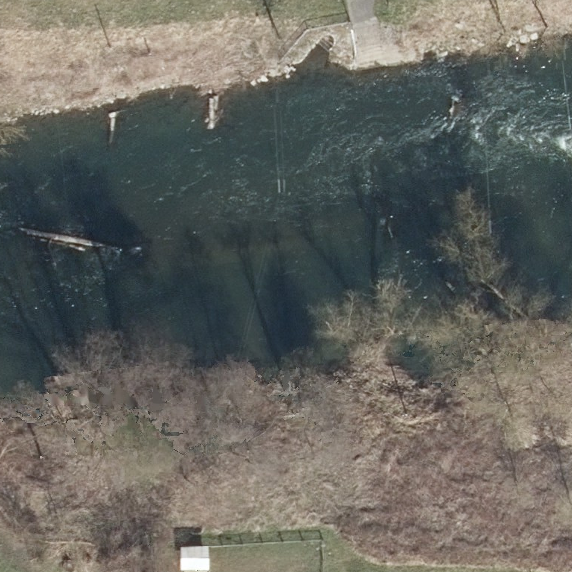
\includegraphics[width=\UnetPredictionsImageWidth]{images/unet/82607-image} \hfill
    
\includegraphics[width=\UnetPredictionsImageWidth]{images/unet/82607-label} \hfill
    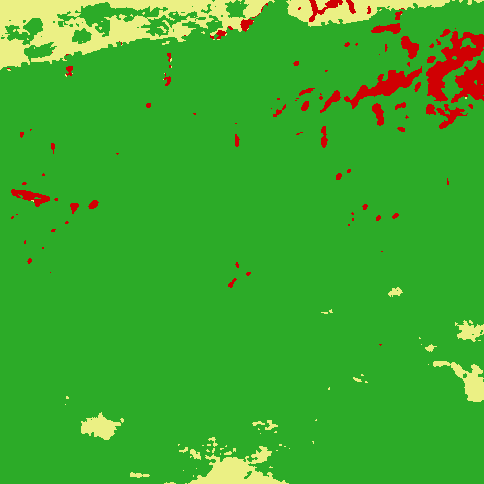
\includegraphics[width=\UnetPredictionsImageWidth]{images/unet/unet-18D/82607-prediction} \hfill
    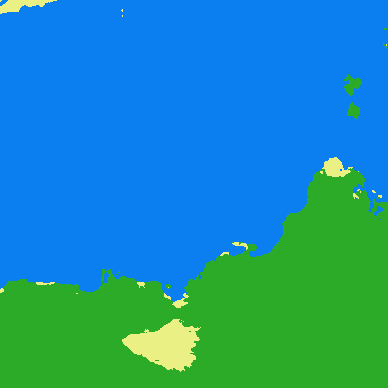
\includegraphics[width=\UnetPredictionsImageWidth]{images/unet/unet-23/82607-prediction} \hfill
    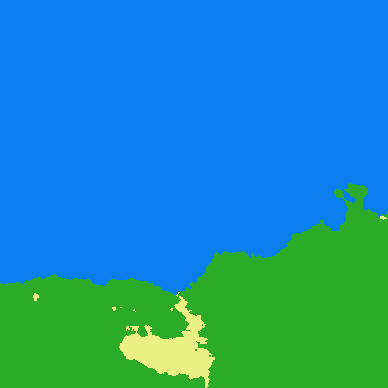
\includegraphics[width=\UnetPredictionsImageWidth]{images/unet/unet-23D/82607-prediction}

    \vspace{3mm}
    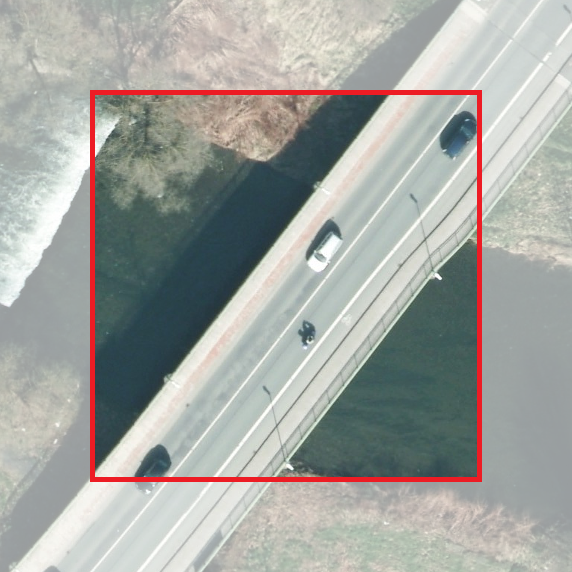
\includegraphics[width=\UnetPredictionsImageWidth]{images/unet/104483-image} \hfill
    
\includegraphics[width=\UnetPredictionsImageWidth]{images/unet/104483-label} \hfill
    
\includegraphics[width=\UnetPredictionsImageWidth]{images/unet/unet-18D/104483-prediction} \hfill
    
\includegraphics[width=\UnetPredictionsImageWidth]{images/unet/unet-23/104483-prediction} \hfill
    
\includegraphics[width=\UnetPredictionsImageWidth]{images/unet/unet-23D/104483-prediction}

    \vspace{3mm}
    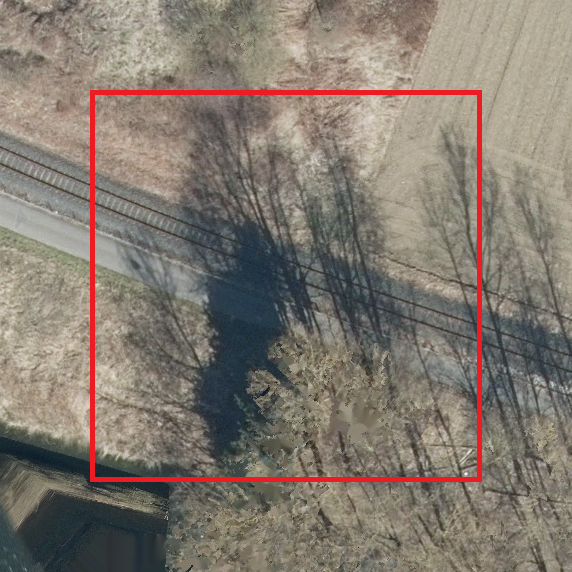
\includegraphics[width=\UnetPredictionsImageWidth]{images/unet/114975-image} \hfill
    
\includegraphics[width=\UnetPredictionsImageWidth]{images/unet/114975-label} \hfill
    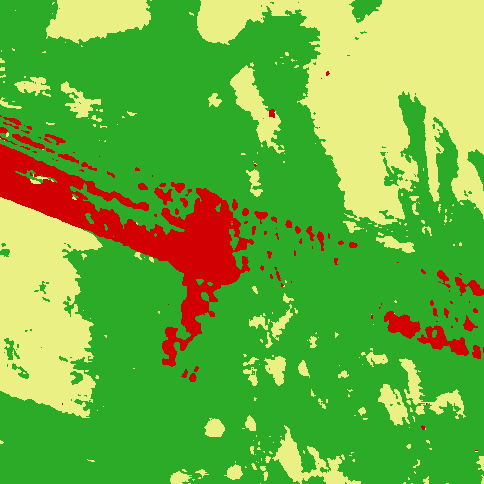
\includegraphics[width=\UnetPredictionsImageWidth]{images/unet/unet-18D/114975-prediction} \hfill
    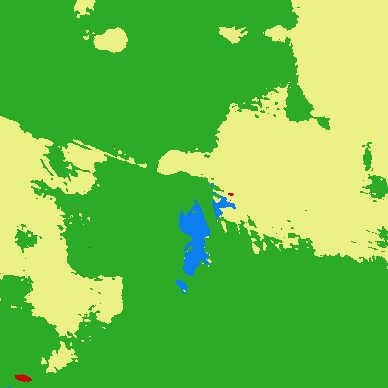
\includegraphics[width=\UnetPredictionsImageWidth]{images/unet/unet-23/114975-prediction} \hfill
    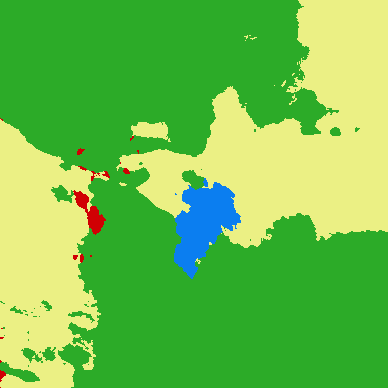
\includegraphics[width=\UnetPredictionsImageWidth]{images/unet/unet-23D/114975-prediction}

    \vspace{3mm}
    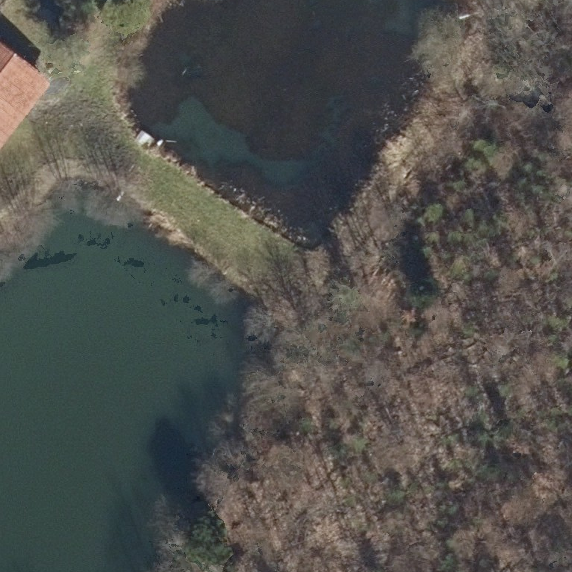
\includegraphics[width=\UnetPredictionsImageWidth]{images/unet/138625-image} \hfill
    
\includegraphics[width=\UnetPredictionsImageWidth]{images/unet/138625-label} \hfill
    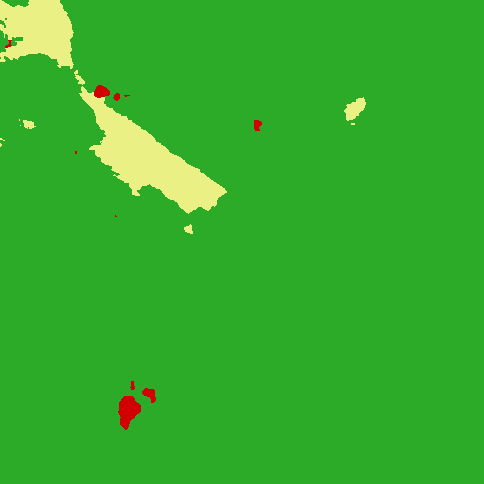
\includegraphics[width=\UnetPredictionsImageWidth]{images/unet/unet-18D/138625-prediction} \hfill
    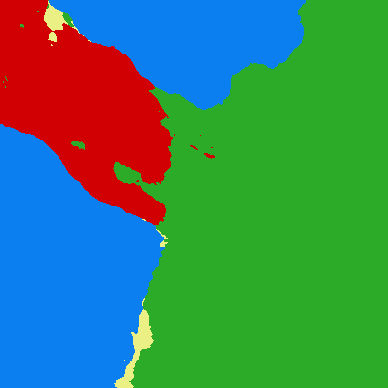
\includegraphics[width=\UnetPredictionsImageWidth]{images/unet/unet-23/138625-prediction} \hfill
    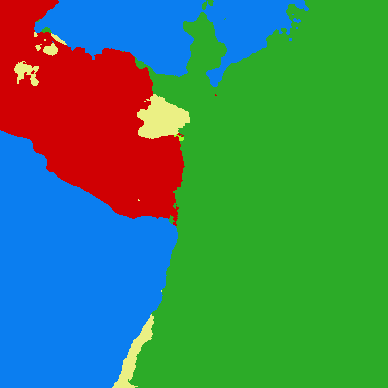
\includegraphics[width=\UnetPredictionsImageWidth]{images/unet/unet-23D/138625-prediction}

    \vspace{3mm}
    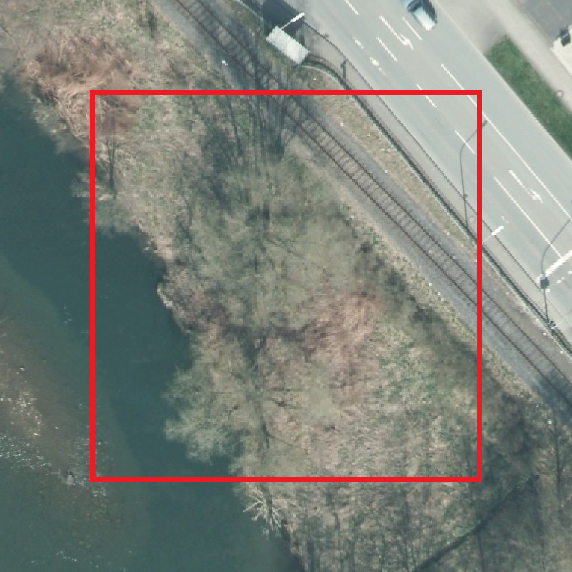
\includegraphics[width=\UnetPredictionsImageWidth]{images/unet/147352-image} \hfill
    
\includegraphics[width=\UnetPredictionsImageWidth]{images/unet/147352-label} \hfill
    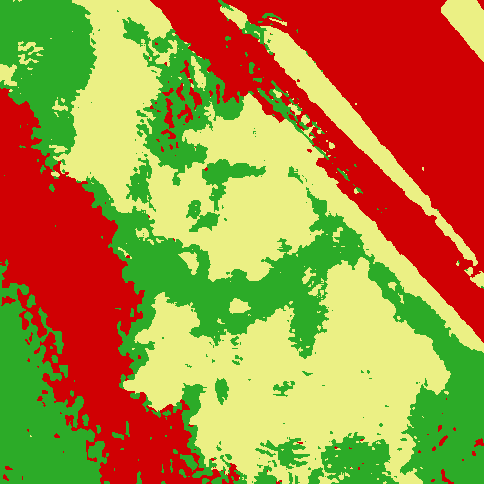
\includegraphics[width=\UnetPredictionsImageWidth]{images/unet/unet-18D/147352-prediction} \hfill
    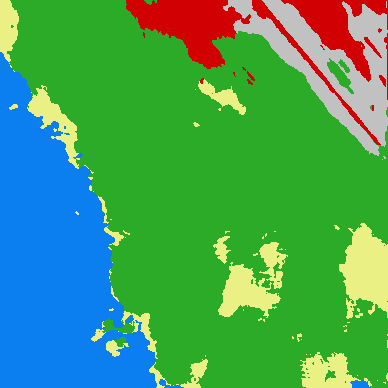
\includegraphics[width=\UnetPredictionsImageWidth]{images/unet/unet-23/147352-prediction} \hfill
    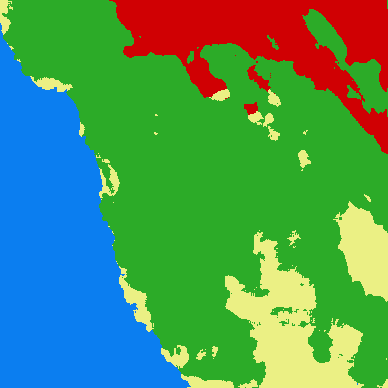
\includegraphics[width=\UnetPredictionsImageWidth]{images/unet/unet-23D/147352-prediction}

    \begin{tikzpicture}
        \node[align=center] at (-1.2, 0) {\tiny Input};
        \node[align=center] at (2.0, 0) {\tiny Ground Truth};
        \node[align=center] at (5.0, 0) {\tiny U-Net-18D};
        \node[align=center] at (8.1, 0) {\tiny U-Net-23};
        \node[align=center] at (11, 0) {\tiny U-Net-23D};
    \end{tikzpicture}
    \caption{Selected predictions of different configurations of U-Net}
    \label{fig:unet_prediction_images}
\end{figure}

The third column of the figure visualizes predictions of the \texttt{U-Net-18D} configuration. The predictions do not contain any \texttt{water} class. Instead, water bodies are predicted to be either \texttt{forest} or \texttt{buildings}. This explains why the categorical accuracy and mean IoU are lower compared to the \texttt{U-Net-23} configurations.

Both \texttt{U-Net-23} and \texttt{U-Net-23D} show better results for the \texttt{water} class. They are able to detect water surfaces correctly. However, sometimes shadows of other objects are also considered to be \texttt{water} (middle row). The first row shows that in some cases the predictions are even better than the labels.

All configurations struggle with the \texttt{traffic} class. In most situations, roads are incorrectly projected to \texttt{buildings}. Only \texttt{U-Net-23} has some correct predictions for the \texttt{traffic} class.

Based on the images shown in figure~\ref{fig:unet_prediction_images}, it is not possible to analyze the predictions with regards to the distinction between \texttt{forest} and \texttt{agriculture}. This will be considered later on in section~\ref{sec:segmentation_discussion}.

\subsection{Experiments with FC-DenseNet}
In the next step, the FC-DenseNet reference architecture is investigated with regards to the segmentation challenge. Again, we analyze the original architecture like described in section~\ref{sec:densenet} as well as some variations with slightly modified hyperparameters.

For this architecture the dimensions of input and output are equally set to $256\times 256$. Since the convolutional layers in this architecture use padding, the dimensions are independent from the number of layers.

The loss is again calculated by a categorical crossentropy function. During training, the weight updates are applied using a RMSprop~\cite{rmsprop14} optimizer. The learning rate is initialized with $0.001$ (according to~\cite{denseseg17}) and decreased after each epoch.

Another naming convention is applied to distinguish the variations of the FC-DenseNet models. The reference model is called \texttt{FCDN-103D}, again indicating the number of convolutional layers and the use of dropout. The letter \texttt{C} denotes the application of compression layers before transition-down layers to condense the outputs of dense blocks (see~\cite{denseseg17} for details). The compression rate of those layers is set to $0.5$, i.~e. the number of feature maps is halved.
% TODO: list configurations, give reasons for them

\subsubsection{Metrics}
The training metrics for all FC-DenseNet configurations are presented in figure~\ref{fig:densenet_train_metrics}. Although there are some strong oscillations, most of the configurations show ongoing improvements over the course of 20 epochs. Towards the end of the training the oscillations faint and the graphs converge.

This behavior is a sign that the initial learning rate was set too high. The weights in the model are then adjusted too drastically, so that minima of the loss function are skipped. The learning rate shrinks towards the end of the training, which explains the reduced oscillations.

According to figure~\ref{fig:densenet_train_metrics}, \texttt{FCDN-103D} yields the best results. At the end of the training the metrics are at a loss of $1.17$, categorical accuracy of $62.6\%$ and mean IoU of $28.4\%$. Those numbers are substantially better than the other configurations, which probably relies on the fact that this configuration also has the highest number of parameters.

The other three configurations report fairly uniform results in terms of metrics. This is very interesting with regards to performance and computational efficiency. \texttt{FCDN-103DC} has more than twice the number of parameters than \texttt{FCDN-56D} ($5.9~\text{M}$ compared to $2.7~\text{M}$) and still many more than \texttt{FCDN-67D} ($4.0~\text{M}$). This means that the configurations with fewer parameters store their information much more efficiently.

\subsubsection{Images}
\WIP{
taking into account the practical usability, it is usefull to look at actual predictions. figure \ref{fig:densenet_prediction_images} shows original image, ground truth and predictions of the models. \texttt{FC-DenseNet-103D}
 predictions are very fragmented for some regions. this indicates that confidence for predictions is rather low. other models do not show so much fragmentation.

From a visual aspect, \texttt{FC-DenseNet-103CD} and \texttt{FC-DenseNet-67D} seem to deliver best results. especially predictions for water are rather nice. However, predictions for traffic are very bad. Not a single model delivers predictions for traffic, all of them confuse it with buildings.
}

\begin{figure}
    \newcommand{\DensenetMetricsImageWidth}{0.32\textwidth}
    \centering
            \begin{scaletikzpicturetowidth}{\textwidth}
\begin{tikzpicture}[scale=\tikzscale]
    \begin{axis}[
        mark=x,
        cycle list name=mycolorlist,
        name=densenetplot1,
        xmin=1, xmax=20,
    ]

    \addplot
    coordinates{
        (1, 1.8778098821640015)
        (2, 1.2668427228927612)
        (3, 1.2766574621200562)
        (4, 1.4314723014831543)
        (5, 1.4286470413208008)
        (6, 1.3057966232299805)
        (7, 1.2254855632781982)
        (8, 1.4993059635162354)
        (9, 1.1675904989242554)
        (10, 1.490395188331604)
        (11, 1.2040382623672485)
        (12, 1.4405009746551514)
        (13, 1.3286089897155762)
        (14, 1.210574984550476)
        (15, 1.1925950050354004)
        (16, 1.3692342042922974)
        (17, 1.2186700105667114)
        (18, 1.2532116174697876)
        (19, 1.1861357688903809)
        (20, 1.168188214302063)
    };

    \addplot
    coordinates{
        (1, 2.1999971866607666)
        (2, 1.3902311325073242)
        (3, 1.3412078619003296)
        (4, 1.2981048822402954)
        (5, 1.280882716178894)
        (6, 1.2695380449295044)
        (7, 1.3394079208374023)
        (8, 1.2355924844741821)
        (9, 1.2429777383804321)
        (10, 1.3308765888214111)
        (11, 1.2678800821304321)
        (12, 1.2725298404693604)
        (13, 1.3483526706695557)
        (14, 1.3196649551391602)
        (15, 1.2746803760528564)
        (16, 1.3376092910766602)
        (17, 1.3442707061767578)
        (18, 1.327423095703125)
        (19, 1.2989463806152344)
        (20, 1.2952357530593872)
    };

    \addplot
    coordinates{
        (1, 2.3974061012268066)
        (2, 1.3469152450561523)
        (3, 1.3552826642990112)
        (4, 1.326025128364563)
        (5, 1.3972184658050537)
        (6, 1.316970944404602)
        (7, 1.295585036277771)
        (8, 1.3838255405426025)
        (9, 1.2869324684143066)
        (10, 1.3071309328079224)
        (11, 1.3551321029663086)
        (12, 1.3308088779449463)
        (13, 1.375392198562622)
        (14, 1.34626042842865)
        (15, 1.3224772214889526)
        (16, 1.3284034729003906)
        (17, 1.3779839277267456)
        (18, 1.3398308753967285)
        (19, 1.3465551137924194)
        (20, 1.3300797939300537)
    };

    \addplot
    coordinates{
        (1, 1.990792155265808)
        (2, 1.294736623764038)
        (3, 1.2612152099609375)
        (4, 1.2450172901153564)
        (5, 1.24184250831604)
        (6, 1.2792901992797852)
        (7, 1.2662909030914307)
        (8, 1.37437903881073)
        (9, 1.2648396492004395)
        (10, 1.2657694816589355)
        (11, 1.316687822341919)
        (12, 1.4254909753799438)
        (13, 1.2919646501541138)
        (14, 1.3055157661437988)
        (15, 1.285273790359497)
        (16, 1.3169896602630615)
        (17, 1.3447442054748535)
        (18, 1.303223967552185)
        (19, 1.2977485656738281)
        (20, 1.2806230783462524)
    };

    \end{axis}
     \begin{axis}[
        mark=x,
        cycle list name=mycolorlist,
        name=densenetplot2,
        at=(densenetplot1.right of south east), anchor=left of south west,
        legend style={at={(0.5,-0.25)},anchor=north},
        xmin=1, xmax=20,
    ]

    \addplot
    coordinates{
        (1, 0.44403234124183655)
        (2, 0.5382390022277832)
        (3, 0.5460906624794006)
        (4, 0.5117834806442261)
        (5, 0.49210643768310547)
        (6, 0.5355142951011658)
        (7, 0.5704494714736938)
        (8, 0.4416641891002655)
        (9, 0.6110737323760986)
        (10, 0.4632301926612854)
        (11, 0.590806782245636)
        (12, 0.5226526260375977)
        (13, 0.5564858317375183)
        (14, 0.5993890166282654)
        (15, 0.613778829574585)
        (16, 0.5397917628288269)
        (17, 0.5880735516548157)
        (18, 0.5896559357643127)
        (19, 0.6149882078170776)
        (20, 0.6262763142585754)
    };
    \addlegendentry{FC-DenseNet-103D}

    \addplot
    coordinates{
        (1, 0.31083741784095764)
        (2, 0.4629298746585846)
        (3, 0.47024381160736084)
        (4, 0.5197407603263855)
        (5, 0.5138208270072937)
        (6, 0.5358591675758362)
        (7, 0.4863249957561493)
        (8, 0.5566446781158447)
        (9, 0.5620558261871338)
        (10, 0.49684542417526245)
        (11, 0.5612539649009705)
        (12, 0.5544501543045044)
        (13, 0.5163871049880981)
        (14, 0.5430474281311035)
        (15, 0.5622951984405518)
        (16, 0.5312788486480713)
        (17, 0.5277349352836609)
        (18, 0.5413538217544556)
        (19, 0.5542507767677307)
        (20, 0.5590786933898926)
    };
    \addlegendentry{FC-DenseNet-103CD}

    \addplot
    coordinates{
        (1, 0.24311639368534088)
        (2, 0.4761204421520233)
        (3, 0.4544506072998047)
        (4, 0.4913800060749054)
        (5, 0.41295066475868225)
        (6, 0.5058783292770386)
        (7, 0.5192673206329346)
        (8, 0.4526740610599518)
        (9, 0.5332894325256348)
        (10, 0.5307732820510864)
        (11, 0.5094674229621887)
        (12, 0.5299655795097351)
        (13, 0.49733099341392517)
        (14, 0.5140370726585388)
        (15, 0.5340467691421509)
        (16, 0.525802493095398)
        (17, 0.499888151884079)
        (18, 0.5290431976318359)
        (19, 0.5265495777130127)
        (20, 0.5373263955116272)
    };
    \addlegendentry{FC-DenseNet-67D}

    \addplot
    coordinates{
        (1, 0.3250448405742645)
        (2, 0.5240246057510376)
        (3, 0.5330521464347839)
        (4, 0.5476676821708679)
        (5, 0.5379430651664734)
        (6, 0.5243373513221741)
        (7, 0.5286471247673035)
        (8, 0.47282737493515015)
        (9, 0.5424470901489258)
        (10, 0.5523974299430847)
        (11, 0.5108893513679504)
        (12, 0.5004795789718628)
        (13, 0.5263856053352356)
        (14, 0.5332449078559875)
        (15, 0.5562388896942139)
        (16, 0.534349262714386)
        (17, 0.5274752974510193)
        (18, 0.5481530427932739)
        (19, 0.5545112490653992)
        (20, 0.5611099600791931)
    };
    \addlegendentry{FC-DenseNet-56D}

    \end{axis}

    \begin{axis}[
        mark=x,
        cycle list name=mycolorlist,
        at=(densenetplot2.right of south east), anchor=left of south west,
        xmin=1, xmax=20,
        ymin=0, ymax=0.35,
    ]

    \addplot
    coordinates{
        (1, 0.15961624681949615)
        (2, 0.23034006357192993)
        (3, 0.2510993778705597)
        (4, 0.2040325254201889)
        (5, 0.15874336659908295)
        (6, 0.2393379658460617)
        (7, 0.2576610743999481)
        (8, 0.20172123610973358)
        (9, 0.28852298855781555)
        (10, 0.1903650313615799)
        (11, 0.2816150486469269)
        (12, 0.2380661964416504)
        (13, 0.2526349425315857)
        (14, 0.28796717524528503)
        (15, 0.29596516489982605)
        (16, 0.2512836754322052)
        (17, 0.2903881371021271)
        (18, 0.28366556763648987)
        (19, 0.30205875635147095)
        (20, 0.28375494480133057)
    };

    \addplot
    coordinates{
        (1, 0.08612015843391418)
        (2, 0.18902510404586792)
        (3, 0.18584029376506805)
        (4, 0.2238929122686386)
        (5, 0.21692800521850586)
        (6, 0.2446306347846985)
        (7, 0.19728021323680878)
        (8, 0.254301518201828)
        (9, 0.2588264048099518)
        (10, 0.21687805652618408)
        (11, 0.2554681599140167)
        (12, 0.24556516110897064)
        (13, 0.21257217228412628)
        (14, 0.23620039224624634)
        (15, 0.23790551722049713)
        (16, 0.2152477353811264)
        (17, 0.2248375415802002)
        (18, 0.2260301262140274)
        (19, 0.2301390916109085)
        (20, 0.240129753947258)
    };

    \addplot
    coordinates{
        (1, 0.05528780445456505)
        (2, 0.2058449238538742)
        (3, 0.1926068663597107)
        (4, 0.1960599273443222)
        (5, 0.1480538696050644)
        (6, 0.21407771110534668)
        (7, 0.22343073785305023)
        (8, 0.1498967856168747)
        (9, 0.21587294340133667)
        (10, 0.23544591665267944)
        (11, 0.21624718606472015)
        (12, 0.21524637937545776)
        (13, 0.1991012543439865)
        (14, 0.2097732275724411)
        (15, 0.2226145714521408)
        (16, 0.21674305200576782)
        (17, 0.21302568912506104)
        (18, 0.21026158332824707)
        (19, 0.22532594203948975)
        (20, 0.23161913454532623)
    };

    \addplot
    coordinates{
        (1, 0.13292203843593597)
        (2, 0.22567109763622284)
        (3, 0.23399783670902252)
        (4, 0.2489478588104248)
        (5, 0.19032984972000122)
        (6, 0.2309076339006424)
        (7, 0.2147936075925827)
        (8, 0.1856151819229126)
        (9, 0.20955342054367065)
        (10, 0.24931295216083527)
        (11, 0.20019109547138214)
        (12, 0.17687444388866425)
        (13, 0.18552462756633759)
        (14, 0.19671611487865448)
        (15, 0.21579863131046295)
        (16, 0.1941973716020584)
        (17, 0.21591031551361084)
        (18, 0.20780526101589203)
        (19, 0.2145579308271408)
        (20, 0.21770614385604858)
    };

    \end{axis}

    \node[align=center] at (3.3, -0.65) {\tiny loss};
    \node[align=center] at (11, -0.65) {\tiny cat. accuracy};
    \node[align=center] at (19, -0.65) {\tiny mean IoU};
\end{tikzpicture}
\end{scaletikzpicturetowidth}

    \caption{Training metrics of different variations of FC-DenseNet}
    \label{fig:densenet_train_metrics}
\end{figure}

\begin{figure}
    \newcommand{\DensenetPredictionsImageWidth}{0.15\textwidth}
    \centering

    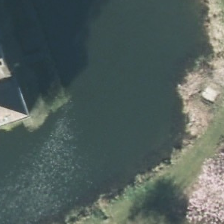
\includegraphics[width=\DensenetPredictionsImageWidth]{images/densenet/101444-image} \hfill
    
\includegraphics[width=\DensenetPredictionsImageWidth]{images/densenet/101444-label} \hfill
    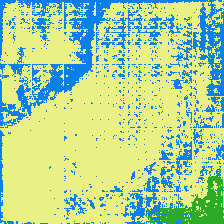
\includegraphics[width=\DensenetPredictionsImageWidth]{images/densenet/densenet-103D/101444-prediction} \hfill
    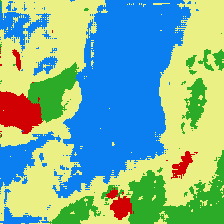
\includegraphics[width=\DensenetPredictionsImageWidth]{images/densenet/densenet-103CD/101444-prediction} \hfill
    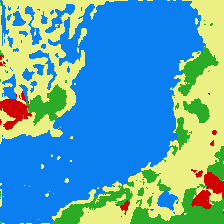
\includegraphics[width=\DensenetPredictionsImageWidth]{images/densenet/densenet-67D/101444-prediction} \hfill
    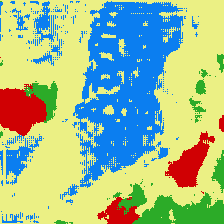
\includegraphics[width=\DensenetPredictionsImageWidth]{images/densenet/densenet-56D/101444-prediction}

    \vspace{3mm}
    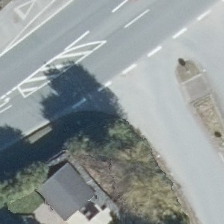
\includegraphics[width=\DensenetPredictionsImageWidth]{images/densenet/291991-image} \hfill
    
\includegraphics[width=\DensenetPredictionsImageWidth]{images/densenet/291991-label} \hfill
    
\includegraphics[width=\DensenetPredictionsImageWidth]{images/densenet/densenet-103D/291991-prediction} \hfill
    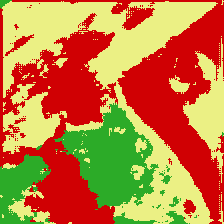
\includegraphics[width=\DensenetPredictionsImageWidth]{images/densenet/densenet-103CD/291991-prediction} \hfill
    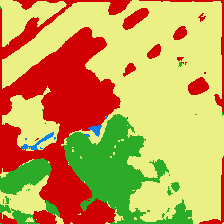
\includegraphics[width=\DensenetPredictionsImageWidth]{images/densenet/densenet-67D/291991-prediction} \hfill
    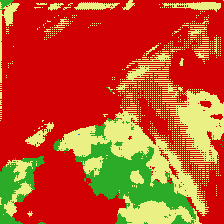
\includegraphics[width=\DensenetPredictionsImageWidth]{images/densenet/densenet-56D/291991-prediction}

    \vspace{3mm}
    \includegraphics[width=\DensenetPredictionsImageWidth]{images/densenet/436897-image} \hfill
    \includegraphics[width=\DensenetPredictionsImageWidth]{images/densenet/436897-label} \hfill
    \includegraphics[width=\DensenetPredictionsImageWidth]{images/densenet/densenet-103D/436897-prediction} \hfill
    \includegraphics[width=\DensenetPredictionsImageWidth]{images/densenet/densenet-103CD/436897-prediction} \hfill
    \includegraphics[width=\DensenetPredictionsImageWidth]{images/densenet/densenet-67D/436897-prediction} \hfill
    \includegraphics[width=\DensenetPredictionsImageWidth]{images/densenet/densenet-56D/436897-prediction}

    \vspace{3mm}
    \includegraphics[width=\DensenetPredictionsImageWidth]{images/densenet/626312-image} \hfill
    \includegraphics[width=\DensenetPredictionsImageWidth]{images/densenet/626312-label} \hfill
    \includegraphics[width=\DensenetPredictionsImageWidth]{images/densenet/densenet-103D/626312-prediction} \hfill
    \includegraphics[width=\DensenetPredictionsImageWidth]{images/densenet/densenet-103CD/626312-prediction} \hfill
    \includegraphics[width=\DensenetPredictionsImageWidth]{images/densenet/densenet-67D/626312-prediction} \hfill
    \includegraphics[width=\DensenetPredictionsImageWidth]{images/densenet/densenet-56D/626312-prediction}

    \vspace{3mm}
    \includegraphics[width=\DensenetPredictionsImageWidth]{images/densenet/768909-image} \hfill
    \includegraphics[width=\DensenetPredictionsImageWidth]{images/densenet/768909-label} \hfill
    \includegraphics[width=\DensenetPredictionsImageWidth]{images/densenet/densenet-103D/768909-prediction} \hfill
    \includegraphics[width=\DensenetPredictionsImageWidth]{images/densenet/densenet-103CD/768909-prediction} \hfill
    \includegraphics[width=\DensenetPredictionsImageWidth]{images/densenet/densenet-67D/768909-prediction} \hfill
    \includegraphics[width=\DensenetPredictionsImageWidth]{images/densenet/densenet-56D/768909-prediction}

    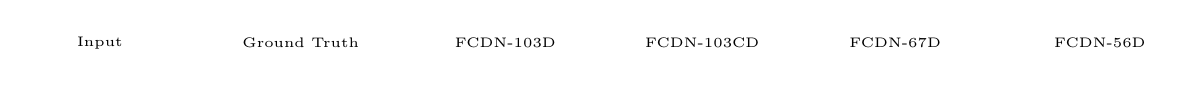
\begin{tikzpicture}
        \node[align=center] at (0, 0) {};
        \node[align=center] at (0.8, 0) {\tiny Input};
        \node[align=center] at (3.35, 0) {\tiny Ground Truth};
        \node[align=center] at (5.95, 0) {\tiny FCDN-103D};
        \node[align=center] at (8.45, 0) {\tiny FCDN-103CD};
        \node[align=center] at (10.9, 0) {\tiny FCDN-67D};
        \node[align=center] at (13.5, 0) {\tiny FCDN-56D};
    \end{tikzpicture}
    \caption{Selected predictions of different configurations of FC-DenseNet}
    \label{fig:densenet_prediction_images}
\end{figure}

\subsection{Experiments with W-Net}
\WIP{
\begin{itemize}
    \item show the architectures of all W-Net models
    \item describe the idea behind the architectural decisions
\end{itemize}
}

\subsection{Discussion}
\label{sec:segmentation_discussion}
\WIP{
\begin{itemize}
    \item have a look at the segments that were found by the NN
    \item show segmentation results of large areas
    \item compare segments to the real landscape in the dataset
    \item discuss practical use of those results for identifying emergency landing fields
    \item evaluate results and assess which data to use for the vegetation analysis
\end{itemize}
}

\newpage

    \section{Analysis of vegetation density}
\label{sec:vegetation_analysis}

\subsection{Spectral Vegetation Indices}
\WIP{
\cite{glv03}
Spectral vegetation indices (SVI) are indicator for vegetation density. based on fact, that healthy vegetation absorbs most of visible red and blue light, but reflect green and NIR light. in fact, reflections of green lights are significantly higher than other spectrums. other materials dont show this bump in green spectrum, instead show steady rise in reflectance as wavelengths increase.

SVIs compare difference between visible and NIR light. the greater the difference, the greater the amount of green vegetation in the scene. There are various indices that each combine data from multiple spectral bands to a single value indicating the vegetation health and density. Most of them use simple algebraic formulas. Some of the commonly used indices are now introduced. 
}

\subsubsection{Ratio Vegetation Index}
\WIP{
\cite{glv03}
Ratio Vegetation Index (RVI) is simply ratio between NIR light and red light (equation \ref{eq:rvi}). Values for non-vegetation area are generally around $1$, because similar reflectance of NIR and red light. index can not go below $0$ for practical reasons (can not be less than no reflectance). Higher means more vegetation, high values typically reaching up to magnitude of $30$. however, there is no upper bound.

\begin{equation}
    \text{RVI} = \frac{\text{NIR}}{\text{Red}}
    \label{eq:rvi}
\end{equation}
}

\subsubsection{Normalized Difference Vegetation Index}
\WIP{
\cite{gisg_ndvi20}
NDVI ranges from $-1$ to $1$. Negative values indicate high probability for water. Positive values imply vegetation, where higher values mean more/denser vegetation. Values around 0 just tell that there is no vegetation, but does not tell about land cover. Could be desert, rocks or urban areas.


\cite{measuring_vegetation00}
first use of vegetation analysis was driven by National Oceanic and Atmospheric Administration (NOAA), US agency focusing on conditions of the environment. They launched satellites carrying an Advanced Very-High-Resolution Radiometer (AVHRR) instrument to measure earth's reflectance in five spectral bands. Two of sensors are sensitive to wavelengths ranging from $550$ to $700$ nanometers (red light), an $730$ to $1000$ nanometers (near-infrared light). the NDVI is based on those two values. \ref{eq:ndvi} shows formula to calculate NDVI.

\begin{equation}
    \text{NDVI} = \frac{\text{NIR}-\text{Red}}{\text{NIR}+\text{Red}}
    \label{eq:ndvi}
\end{equation}
}

\subsection{Building the Neural Network}
\WIP{
\begin{itemize}
    \item show the chosen architectures of all tested models
    \item describe the idea behind the architectural decisions
    \item analyze how the NN works internally (e. g. visualize feature/confidence maps)
    \item explain the data format for the resulting database
\end{itemize}
}

\subsection{Discussion}
\WIP{
\begin{itemize}
    \item compare results to the real landscape in the dataset
    \item discuss practical use of those results for identifying emergency landing fields
\end{itemize}
}

\newpage

    %\section{(Optional) Identification of tractor lane orientation}
% TODO: decide if this section fits the scope of the thesis

\subsection{Preparing the dataset}

\subsection{Training the Neural Network}

\subsection{Discussion}

\newpage

    \section{On the Deployment for Practical Use}
\begin{itemize}
    \item Thoughts how to provide the trained models for practical use.
    \item design of an API?
    \item packaging into a docker image?
\end{itemize}

\newpage

    \section{Conclusion}
The main objective of this thesis was to advance the identification of emergency landing fields with the given dataset. This goal was achieved by a variety of approaches.

For the semantic segmentation of terrain types, three renowned reference architectures have been studied thoroughly. Each architecture was analyzed and presented in detail. The architectures were tested extensively with regards to the segmentation challenge.

The experiments proved that the W-Net architecture is ineffective on the given dataset. The unsupervised training approach generated no new insights on the data and did not lead to a adequate differentiation of class segments. For that reason, it is recommended to not conduct further research on this architecture in the given context.

By contrast, both U-Net and FC-DenseNet architectures have shown great success for the class segmentation. The predictions of U-Net were more contiguous and therefore closer to the labels used for training. On the other hand, the predictions of FC-DenseNet are closer to reality, because they represent very detailed segments. 

Both architectures expose some shortcomings with respect to the underrepresented classes in the dataset. It is recommended to address these issues before installing the models in a production environment. This is likely to be related to the concerns expressed about the inaccurate labels used for training. Therefore, it is recommended to employ a different set of labels for future research. Since manual labelling of the entire dataset comes with very high efforts, another predefined set of labels has to be found. It is also possible to combine information from different sources for  this purpose.

The second objective of the thesis was to evaluate the use of spectral vegetation indices to estimate the density of vegetation. It was discussed in detail to which extent the projections of the SVIs can be use to assess the suitability of areas for emergency landings. In this regard, several indices were reviewed.

Experiments with the indices have shown very inconsistent results. The areas where dense vegetation is predicted differ based on the index that is used. This is unexpected, because even if the indices use different characteristics of the dataset, they should still deliver similar results. One issue with this is, that the dataset itself is lacking precise information about the vegetation itself. Thus the real vegetation density can only be estimated based on the DOPs.

Most of the vegetation indices are designed and calibrated for the use with very specific hardware under very specific conditions. The dataset used in this thesis does not match these conditions. This might explain the inconsistent projections seen across the indices.

Considering all the facts, no clear conclusion can be drawn about the use of vegetation indices. Further research is required to obtain meaningful recommendations on that topic. For that, more information about the real vegetation situation has to be considered together with the indices. By doing that, it is possible to assess which vegetation index best reflects the real vegetation conditions.

In summary, this thesis laid out the foundations to support the identification of emergency landing fields with convolutional neural networks. It is shown that semantic segmentation of terrain types is generally possible with that approach. Further research can build upon this thesis in order to further improve the designed methods.

\clearpage

    \appendix
    \section{Tools and Hardware}
\label{app:tools_hardware}
\noindent
All processing steps and computations were performed on a machine with the following specifications:
\begin{itemize}
    \item Intel Core i7 8700K $6\times$ 3.70 GHz
    \item DDR4-2400 RAM 32 GB
    \item GeForce GTX 1080 Ti (11 GB VRAM)
    \item Samsung SSD 860 EVO 500 GB
    \item Windows 10 (Version 2004)
\end{itemize}

\vspace{8pt}

\noindent
The following table lists all used software packages with their respective purpose in the thesis. \\

\centering{
\resizebox{0.9\textwidth}{!}{%
\begin{tabular}{|l|l|l|}
\hline
Software & Version & Used For \\ \hline \hline
Python & 3.6.8 & Data Pre- and Postprocessing, Implementation of CNNs \\ \hline
Keras (pip-package) & 3.2.1 & Implementation of the CNNs \\ \hline
Tensorflow-GPU (pip-package) & 2.2.0 & Computation Backend for Keras \\ \hline
NumPy (pip-package) & 1.18.4 & Efficient Array Modifications \\ \hline
PsycoPG (pip-package) & 2.8.5 & Access to PostgreSQL-Database \\ \hline
OpenCV (pip-package) & 4.2.0.34 & Read, Modify and Save Images \\ \hline \hline
PostgreSQL & 12.2 & Central Database \\ \hline
postGIS & 3.0 & \begin{tabular}[c]{@{}l@{}}Extension for PostgreSQL, \\ Support for Geospatial Data\end{tabular} \\ \hline \hline
QGIS & 3.12.2 & Visualize and Render Geospatial Data \\ \hline
\end{tabular}%
}
}

    \clearpage
    \phantomsection
    \addcontentsline{toc}{section}{References}
    \bibliography{references}{}
    \bibliographystyle{plain}

    \declarationofauthorship{\WIP{31.10.2020}}
\end{document}
